%% This is file `DEMO-TUDaThesis.tex' version 1.20-beta (2019/10/21),
%% it is part of
%% TUDa-CI -- Corporate Design for TU Darmstadt
%% ----------------------------------------------------------------------------
%%
%%  Copyright (C) 2018--2019 by Marei Peischl <marei@peitex.de>
%%
%% ============================================================================
%% This work may be distributed and/or modified under the
%% conditions of the LaTeX Project Public License, either version 1.3c
%% of this license or (at your option) any later version.
%% The latest version of this license is in
%% http://www.latex-project.org/lppl.txt
%% and version 1.3c or later is part of all distributions of LaTeX
%% version 2008/05/04 or later.
%%
%% This work has the LPPL maintenance status `maintained'.
%%
%% The Current Maintainers of this work are
%%   Marei Peischl <tuda-ci@peitex.de>
%%   Markus Lazanowski <latex@ce.tu-darmstadt.de>
%%
%% The development respository can be found at
%% https://github.com/tudace/tuda_latex_templates
%% Please use the issue tracker for feedback!
%%
%% ============================================================================
%%
% !TeX program = lualatex
%%

\documentclass[
	ngerman,
	ruledheaders=section,%Ebene bis zu der die Überschriften mit Linien abgetrennt werden, vgl. DEMO-TUDaPub
	class=report,% Basisdokumentenklasse. Wählt die Korrespondierende KOMA-Script Klasse
	thesis={type=master},% Dokumententyp Thesis, für Dissertationen siehe die Demo-Datei DEMO-TUDaPhd
	accentcolor=9c,% Auswahl der Akzentfarbe
	custommargins=geometry,% Ränder werden mithilfe von typearea automatisch berechnet
	marginpar=false,% Kopfzeile und Fußzeile erstrecken sich nicht über die Randnotizspalte
	BCOR=10mm,%Bindekorrektur, falls notwendig
	parskip=half-,%Absatzkennzeichnung durch Abstand vgl. KOMA-Sript
	fontsize=11pt,%Basisschriftgröße laut Corporate Design ist mit 9pt häufig zu klein
	colorback=false, % Schaltet zwischen dem farbigen Block auf der Titelseite und weißem Hintergrund um
	bibliography=totoc, % bibliography in toc
	listof=totoc % list of X in toc
%	logofile=example-image, %Falls die Logo Dateien nicht vorliegen
]{tudapub}

%change margins
\geometry{a4paper}


% Der folgende Block ist nur bei pdfTeX auf Versionen vor April 2018 notwendig
\usepackage{iftex}
\ifPDFTeX
\usepackage[utf8]{inputenc}%kompatibilität mit TeX Versionen vor April 2018
\fi

%%%%%%%%%%%%%%%%%%%
%Sprachanpassung & Verbesserte Trennregeln
%%%%%%%%%%%%%%%%%%%
\usepackage[english, main=english]{babel}
\usepackage[autostyle]{csquotes}% Anführungszeichen vereinfacht
\usepackage{microtype}


%%%%%%%%%%%%%%%%%%%
%Literaturverzeichnis
%%%%%%%%%%%%%%%%%%%
\usepackage{biblatex}   % Literaturverzeichnis
\bibliography{bibliography}


%%%%%%%%%%%%%%%%%%%
%Tabellen
%%%%%%%%%%%%%%%%%%%
%\usepackage{array}     % Basispaket für Tabellenkonfiguration, wird von den folgenden automatisch geladen
\usepackage{tabularx}   % Tabellen, die sich automatisch der Breite anpassen
%\usepackage{longtable} % Mehrseitige Tabellen
%\usepackage{xltabular} % Mehrseitige Tabellen mit anpassarer Breite
\usepackage{booktabs}   % Verbesserte Möglichkeiten für Tabellenlayout über horizontale Linien
\usepackage{multirow}
\usepackage{ltablex} % combine the features of the tabularx package (auto-sized columns in a fixed width table) with those of the longtable package (multi-page tables).

%%%%%%%%%%%%%%%%%%%
% Custom packages
%%%%%%%%%%%%%%%%%%%
%\usepackage{mathtools} % erweiterte Fassung von amsmath
%\usepackage{amssymb}   % erweiterter Zeichensatz
%\usepackage{siunitx}   % Einheiten
\usepackage[center,labelfont=bf]{caption}
\usepackage{subfig} % make it possible to include more than one captioned figure/table in a single float
\usepackage{graphicx} % support the \includegraphics command and options
\usepackage{array} % for better arrays (eg matrices) in maths
\usepackage{paralist} % very flexible & customisable lists (eg. enumerate/itemize, etc.)
\usepackage{verbatim} % adds environment for commenting out blocks of text & for better verbatim
\usepackage{float}
\usepackage{amsmath}
\usepackage{acronym}

\usepackage{hyperref} % Hyperlinks
\usepackage[toc]{appendix} % Appendices (also shown in toc)
\usepackage{amsthm} %Typesetting theorems

\usepackage[linesnumbered,ruled]{algorithm2e}
\usepackage{enumitem}

\usepackage{blindtext} % to generate dummy text for the example

% sets the default path for images
\graphicspath{{img/}}

%Formatierungen für Beispiele in diesem Dokument. Im Allgemeinen nicht notwendig!
\let\file\texttt
\let\code\texttt

\begin{document}

\Metadata{
	title=A Learned Advisor for Automated Materialized View Selection,
	author=Michael Girges
}

\title{A Learned Advisor for Automated Materialized View Selection}
\subtitle{}
\author[Signature]{Michael Girges}%optionales Argument ist die Signatur, 
\reviewer{Prof. Dr. Carsten Binnig \and Johannes Wehrstein \and Roman Heinrich}%Gutachter

%Diese Felder erden untereinander auf der Titelseite platziert. 
%\department ist eine notwendige Angabe, siehe auch dem Abschnitt `Abweichung von den Vorgaben für die Titelseite'
\department{inf} % Das Kürzel wird automatisch ersetzt und als Studienfach gewählt, siehe Liste der Kürzel im Dokument.
\institute{Data Management Lab}
\addTitleBoxLogo{dm_logo}
\submissiondate{\today}
\examdate{\today}

%	\tuprints{urn=1234,printid=12345}
%	\dedication{Für alle, die \TeX{} nutzen.}

\maketitle

% erzeugt eine Selbstständigkeitserklärung mit Unterschriftenzeile.
\affidavit

% insert abstract before contents
\begin{abstract}
    
\ac{MV} are commonly used in databases to accelerate read queries, but their benefits come with high maintenance costs and full refreshes to avoid stale data. \ac{IMV} offer an alternative by updating views incrementally through triggers. However, they perform best in read-heavy workloads and may introduce significant write-time overhead. This work proposes a machine-learning-based advisor that, given a SQL workload, predicts whether to use \ac{MV}, \ac{IMV}, or no views at all for optimal performance. The advisor jointly considers the cost of maintaining views during writes and the potential performance gains during reads. Our approach aims to guide database administrators and automated tuning systems in selecting the most effective view strategy based on workload characteristics.

\end{abstract}







% create the table of contents
\tableofcontents

% List of figures (Abbildungsverzeichnis):
\listoffigures


\chapter*{List of Abbreviations}
\addcontentsline{toc}{chapter}{List of Abbreviations}

\begin{acronym}
\acro{API}{Ap\-pli\-ca\-tion Programming Interface}		
\acro{DBMS}{Database Management System}		
\acro{MV}{Materialized View}
\acro{IMV}{Incremental Materialized View}
\acro{IVM}{Incremental View Maintenance}
\acro{DML}{Data Manipulation Language}
\acro{ML}{Machine Learning}
\acro{ILP}{Integer Linear Programming}
\acro{DTA}{Database Tuning Advisor}
\acro{T3}{Tuple Time Tree}
\acro{QEP}{Query Execution Plan}
\end{acronym}
\chapter{Introduction}
\label{chap:introduction}
\IMRADlabel{introduction} % Mechanismus um das Strukturierungsmodell IMRaD zu kennzeichnen
% Recipe for a good introduction (LeanStore)
    %How are things done before new HW (pre main-memory db)
    %Motivate why the way it was done is suboptimal
    %Visually illustrate the suboptimality
    %Include related approaches and state suboptimality
    %Motivate further by hardware trends
    %Raise fundamental question for paper
    %Give short overview of contribution and result (abstract-like)


\section{Context and Motivation}
\label{sec:context}
\ac{MV}s are a common optimization in database systems: by precomputing and storing query results they can substantially accelerate read queries. However, materialized views introduce maintenance costs whenever base tables change, because the view contents must be kept consistent with the underlying data. The naive strategy of full recomputation can become prohibitively expensive for workloads with frequent updates.

Incrementally maintained materialized views (\ac{IMV}s) provide an alternative maintenance strategy by applying only the changes (deltas) caused by updates to base tables, instead of recomputing entire views. \ac{IMV}s can significantly reduce maintenance work for many workloads, but they are not a universal win: their benefit depends on workload characteristics. In particular, \ac{IMV}s tend to be most advantageous for read-heavy workloads with relatively small or structured updates, while write-heavy workloads can cause high incremental maintenance overhead and complex update propagation.

Choosing between no views, conventional \ac{MV}s, and \ac{IMV}s therefore requires trading off read-performance gains against the cost of maintaining views under updates. Manually exploring this trade-off is time-consuming and error-prone. This thesis proposes to automate that decision by building a machine learning-based advisor that, given a SQL workload composed of reads and writes, recommends the view strategy that is likely to be optimal in terms of overall system performance and maintenance cost.

\section{Problem Statement}
\label{sec:problemStatment}
The central problem addressed in this work is:

\begin{quote}
Given a SQL workload (a sequence or distribution of read and write statements) and information about the database/schema, determine whether the workload is best served by (i) no materialized views, (ii) materialized views with full recomputation, or (iii) incrementally maintained materialized views (\ac{IMV}s), taking into account both query performance and view maintenance costs.
\end{quote}

Concretely, this requires (a) modelling the costs and benefits of each strategy for a given workload, and (b) designing a predictor that maps workload characteristics to the recommended strategy. To support cost-aware decision making, this thesis includes the design of a write-cost estimation model inspired by decision-tree approaches (cf.\ the T3 system\cite{rieger2025t3}).

This thesis answers the following research questions:

\begin{enumerate}
    \item When is it beneficial to use \ac{MV}, \ac{IMV}, or no materialized view at all for a given SQL workload?
    \item Can a machine learning model accurately and efficiently predict the optimal view strategy for a workload based on its read and write characteristics?
\end{enumerate}

\section{Goals and Contributions}
\label{sec:goals}
The goals of this thesis are to design, implement, and evaluate an automated advisor that recommends one of the three view strategies (no view, \ac{MV}, or \ac{IMV}) for a given SQL workload. The primary contributions are:

\begin{itemize}
    \item The design of a machine learning-based advisor that takes workload features as input and outputs a recommended view strategy (no view / \ac{MV} / \ac{IMV}).
    \item A cost estimation component for write operations that informs the advisor; this component leverages a decision-tree-based approach inspired by the T3 system\cite{rieger2025t3}.
    \item An empirical evaluation demonstrating the advisor's effectiveness at selecting strategies that balance read performance and maintenance overhead across a variety of workloads.
\end{itemize}

\section{Thesis Outline}
\label{sec:outline}
The remainder of the thesis is organized as follows:

\begin{itemize}
    \item Chapter~\ref{chap:background} presents background material and related work on materialized views, incremental maintenance techniques, and workload-aware tuning approaches.
    \item Chapter~\ref{chap:design} describes the design of the ML advisor, including the workload feature representation and the cost estimation model for writes.
    \item Chapter~\ref{chap:implementation} details the implementation decisions and integration with the chosen database/testing infrastructure.
    \item Chapter~\ref{chap:evaluation} reports the experimental methodology and results evaluating prediction accuracy and overall performance impact of the recommended strategies.
    \item Chapter~\ref{chap:conclusion_futurework} concludes the thesis, summarizes findings, and outlines directions for future work.
\end{itemize}

\chapter{Background}
\label{chap:background}

\section{Automated View Selection}
\label{sec:related_work}

Automated database tuning, notably the selection and management of physical design structures such as \ac{MV}s and indexes, has long been a critical and challenging task for database administrators. Traditional approaches often rely on manual expertise \cite{yuan2020automatic} or on complex rule-based and enumeration-based heuristics, which become particularly cumbersome for rich \ac{MV} structures or complex queries \cite{ahmed2020automated}.

Early automated \ac{MV} selection work explored heuristic systems that choose candidate views based on estimated cost and validate them against the actual database \cite{ahmed2020automated}. Commercial systems like Microsoft SQL Server's \ac{DTA} provide workload-driven recommendations for indexes and \ac{MV}s \cite{ahmed2020automated}. Other research formulates view selection as an optimization problem (for example, \ac{ILP}) \cite{yuan2020automatic}; while these formulations can be precise, they are often computationally expensive for large sets of subqueries or extensive workloads, and iterative methods may not guarantee convergence.

More recently, \ac{ML} methods have been applied to a variety of database tasks with the goal of replacing handcrafted components by learned models that can automatically handle complexity and variability \cite{kossmann2022swirl, hilprecht2020learning}. A common paradigm in learned database components is workload-driven learning, which typically requires executing representative workloads on the target database to collect training data. Although effective in many settings, this data-collection step is costly and must often be repeated for each new database or substantially changed workload \cite{kossmann2022swirl}. To address this limitation, zero-shot learning approaches have emerged: models are pretrained once and designed to generalize to unseen databases or workloads without per-database retraining. Initial zero-shot work has focused on tasks such as cost estimation \cite{sun2019end}, and researchers are investigating extensions of this paradigm to tasks like \ac{MV} selection.

The maintenance of \ac{MV}s - especially incremental maintenance - is another important axis in the literature. For example, commercial systems include refresh/maintenance modules that track refresh methods and schedules; some research and product directions explore using \ac{ML} to predict refresh behavior or maintenance cost and to incorporate those predictions into recommendation logic \cite{ahmed2020automated}. This line of work suggests that predicted maintenance cost (including incremental refresh cost) can and should influence which views are recommended. The interaction between specific maintenance strategies (e.g., incremental refresh) and \ac{ML}-based recommendation processes remains an active area where further research can provide valuable insights.

\section{Query Performance Prediction Using Cost Models}
\label{sec:query_performance_prediction}
Accurate query performance prediction is essential for effective physical design tuning, including \ac{MV} selection. Traditional cost models, such as those used in query optimizers, estimate query execution time based on factors like I/O costs, CPU costs, and network costs \cite{selinger1979access}. However, these models often struggle to capture the complexities of modern database systems and workloads, leading to inaccuracies in performance predictions. The first cost model was proposed by Listgarten et al. \cite{listgarten1997cost} as part of their work on main memory databases. Moreover, a framework for building cost models for hierarchical database systems was introduced by Manegold et al.\cite{manegold2002generic}.

In the last couple of decades, learning-based techniques have been increasingly applied to the problem of query performance prediction. Gupta et al. pioneered the use of machine learning for query performance prediction by introducing a decision tree-based approach to predict query execution time ranges\cite{gupta2008pqr}. Query performance prediction has also been approached for static and dynamic workloads using regression models \cite{akdere2012learning}, who implemented these techniques on top of PostgreSQL. Calibration of existing cost models in PostgreSQL has been explored by Wu et al. \cite{wu2013predicting}, where they used small calibration workloasds to adjust the cost model parameters. In combination with an analytical model, they were able to predict the query execution time for larger workloads\cite{wu2013towards}. This approach proved competitive to other contemporary learning-based methods.

Neural networks and deep learning techniques have also been employed for query performance prediction through feeding the tree-structured query plans into neural network architectures. For instance, Sun et al. \cite{sun2019end} concluded that combining tree nodes is effectively handled using a pooling architecture. Zhou et al. proposed encoding single and multiple concurrent queries using a graph embedding approach \cite{zhou2020query}. This approach captures the interactions between concurrent queries and enables accurate predictions of execution times of whole workloads. Additionally, transformer-based architectures and augmenting the input data with database statistics have been shown to further improve prediction accuracy \cite{zhao2022queryformer}.

Since workload-based models do not work well in zero-shot settings, recent research has focused on developing zero-shot query performance prediction models. The first zero-shot query performance prediction model was proposed by Hilprecht et al. \cite{hilprecht2022zero}. Their zero-shot model was trained and evaluated on different databases and workloads, demonstrating the ability to generalize to unseen databases without retraining. More recently, Wu et al. \cite{wu2024stage} introduced a zero-shot model that is trained on the complete Redshift workload. They propose a hierarchical model in an effort to improve latency.

Learning-based approaches have shown promising results in query performance prediction, but they are often criticized in literature for their high end-to-end latency. This latency can be a significant drawback in scenarios where quick predictions are essential for decision-making. Lehmann et al. \cite{lehmann2023your} commented on this issue by concluding that learning-based query optimizers have high optimization times, which renders them impractical for real-world usage. One approach to mitigate this issue is proposed by Wu et al. \cite{wu2024stage}, where they use a query cache with a fallback to a local decision tree model to reduce the end-to-end latency of their zero-shot model.

Other non-learning-based approaches have been proposed to solve the query performance prediction problem. Since these approaches are not dependent on neural networks, they can be more interpretable and can be quicker to train and evaluate. For instance, cost models based on differential programming have been proposed by Hilprecht et al. \cite{hilprecht2020dbms}. They depend on learning some of the constants in pre-existing cost model functions. Another approach is to use different groups of calibration constants for the fixed cost functions in the PostgreSQL cost model \cite{yang2023rethinking}. 

% TODO: write about t3 here and how low-latency it is
\subsection{Tuple Time Tree (T3) Cost Model}
Rieger et al. proposed the \ac{T3} cost model \cite{rieger2025t3}, which bridges the gap between high-accuracy, high-latency learning-based models and their lower-accuracy, low-latency counterparts. \ac{T3} is a hybrid cost model that combines a low-latency decision tree with pipeline-based query plan presentation and tuple-centric prediction targets.

The pipeline-based query plan representation divides the query plan into multiple pipelines, where each pipeline consists of a sequence of operators that can be executed without materializing intermediate results. This representation allows \ac{T3} to generate a flat feature vector for each pipeline and predicts its execution time individually. The total query execution time is calculated as the sum of all pipeline predictions.

On the other hand, tuple-centric prediction is based on the idea that, instead of predicting the total execution time for a pipeline, \ac{T3} predicts the expected time it takes to process a single tuple within that pipeline. Then, the per-tuple time is multiplied by the pipeline's input cardinality to estimate the total execution time of the pipeline. This approach is highly compatible with the decision tree architecture and is highly-scalable.

Furthermore, \ac{T3} improves inference time by compiling the trained model directly into native machine code using the \texttt{lleaves} framework. This step drastically reduces the average prediction latency from 22µs in interpreted trees and 1ms in zero-shot neural networks down to 4 microseconds.

\section{Workload Generation}
\label{sec:workload_generation}
In this work, we require a diverse set of training and evaluation workloads to train and assess our proposed models. Workload generation is a well-researched area, with various methods proposed to create synthetic workloads that mimic real-world query patterns. For example, Kipf et al. \cite{kipf2018learned} introduced a method for generating synthetic SQL queries based on schema information and sampling values from the underlying data. Hilprecht et al. \cite{hilprecht2022zero} built on this approach by enabling the generation of more complex queries that might include joins, random index creation and predicates with null comparison, regex-based string comparison and disjunctions. Additionally, in the Master's thesis "Caching Strategies based on realistic Workloads," Martin Stemmer \cite{Stemmer2025} investigates the practical, cost-based trade-off between full result caching and incremental updates in modern data warehouses. 

\chapter{Methodology}
\label{chap:methodology}
\IMRADlabel{methods}

This chapter details the methodology used to build the \ac{ML}-based zero-shot view advisor. The primary objective is to create an advisor that can predict the optimal view strategy (no view, \ac{MV}, or \ac{IMV}) for a given SQL workload using execution time predictions of SELECT and \ac{DML} execution plans from specialized \ac{T3} cost models. This is achieved by first curating a comprehensive training dataset by executing workloads and capturing their performance, then using this dataset to train a predictive cost model. The trained model is then integrated into a view advisor framework that analyzes workloads and recommends the best view configuration based on predicted costs and benefits.

\section{Training Data Curation}
\label{sec:data_curation}
The foundation of the \ac{ML} advisor is a labeled dataset of query execution times. This dataset must capture performance metrics for both SELECT and \ac{DML} statements in the \ac{IMV} configuration. The phases mentioned below are repeated for 19 out of the 20 databases in the Amazon Redshift dataset \cite{gupta2015amazon}, with the IMDB database being excluded to be used in evaluating the zero-shot model.

\subsection{Dataset and Workload Generation}
\label{sec:dataset_generation}
To build a robust model, we require a diverse set of training and evaluation workloads. We generate synthetic workloads that mimic the characteristics of real-world scenarios, such as the query distributions and read/write mixes found in datasets like the Amazon Redshift workload \cite{gupta2015amazon}.

The data generation involves generating synthetic \texttt{SELECT} queries (read workload) using the parameters in Table~\ref{tab:workload_params}. Additionally, we generate synthetic \ac{DML} statements (write workload) from a curated month-long snippet of the Amazon Redshift dataset using Stemmer's workload generator \cite{Stemmer2025}. Both synthetic workloads' statements are verified syntactically. The workloads are also normalized by cleaning any database sharding suffixes in table names. Following that, we generate matches between the the cleaned read and write workloads. The generated matches are divided into tiny workloads (also called "experiments") that consist of one SELECT statement and its corresponding \ac{DML} queries. The structure of a single experiment is illustrated in Figure~\ref{fig:experiment_diagram}, while the overall workload structure is shown in Figure~\ref{fig:workload_diagram}. 

% single experiment diagram
\begin{figure}[h]
    \centering
    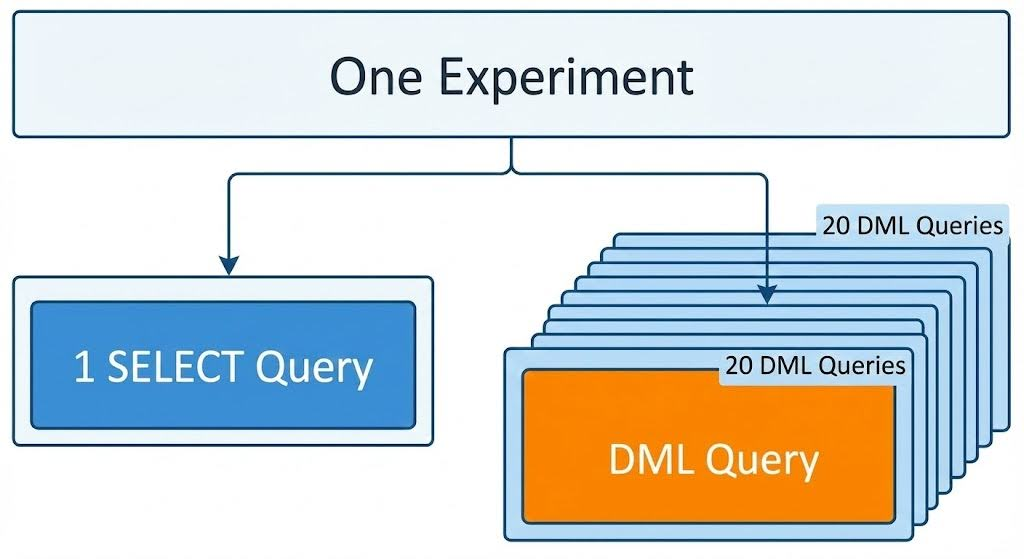
\includegraphics[width=0.8\textwidth]{single-experiment.jpg}
    \caption{Structure of a Single Experiment in the Workload}
    \label{fig:experiment_diagram}
\end{figure}

The matching between SELECT and \ac{DML} queries is based on common base tables they operate on. In each experiment, the maximum number of queries is capped at 1 SELECT and 20 \ac{DML} queries. The total number of queries in all generated experiments is capped at 100,000 queries. This is to ensure manageable execution times while still capturing sufficient variability.

% entire workload diagram
\begin{figure}[h]
    \centering
    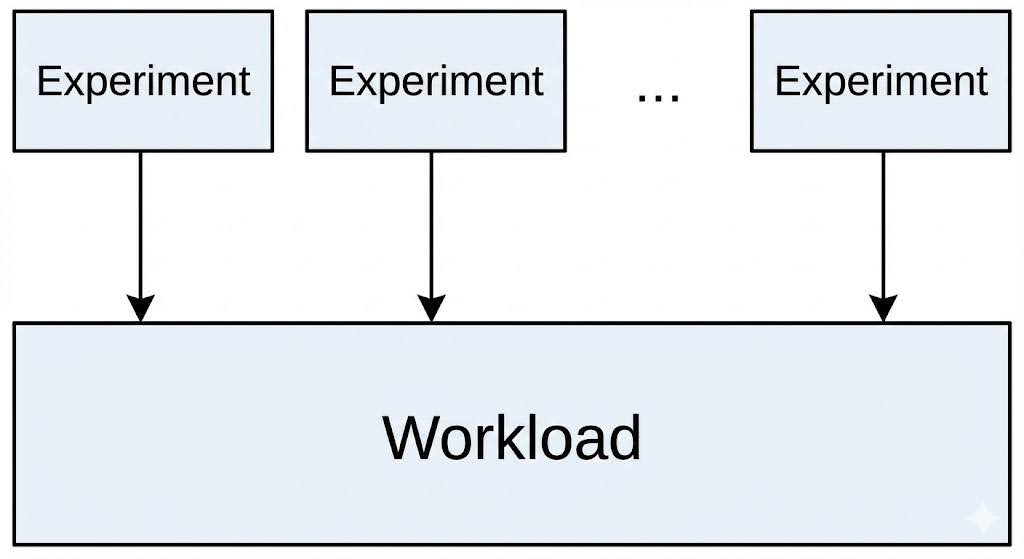
\includegraphics[width=0.8\textwidth]{experiment-workload.jpg}
    \caption{Structure of the Entire Workload Composed of Multiple Experiments}
    \label{fig:workload_diagram}
\end{figure}

\subsection{Experiment Data Collection}
\label{sec:data_collection}
For each defined "experiment" workload, we execute the workload on the target database system under controlled conditions. This instrumentation is critical for capturing the ground-truth performance data.

Preparing the execution environment involves loading the schema and data, the creation of necessary indexes and loading of the necessary extensions--most importantly, the \texttt{pg\_ivm} extension for \ac{IMV} support. Staging tables are used to restore the database state between experiments to ensure consistency. The base tables are loaded as a 10\% sample of the staging tables before each experiment execution. This is to ensure that the \ac{DML} queries have data to operate on while avoiding conflicts with existing table rows. To avoid any cold start scenarios, the database is warmed up before execution. Each experiment is executed only in the \ac{IMV} configuration to capture the relevant performance metrics for both reads and writes.

Each experiment execution consists of the following steps:
\begin{enumerate}
    \item \textbf{Create the \ac{IMV} for the read query:} For the read query in the experiment, we create an \ac{IMV}. This sets up the necessary triggers and structures for incremental maintenance.
    \item \textbf{Execute write queries and measure execution time:} Each \ac{DML} query in the experiment is executed, and its execution time is measured. This captures the "trigger time overhead," which is the \emph{view maintenance cost} incurred by the \ac{IMV} triggers during writes.
\end{enumerate}

This process produces a labeled dataset where each entry includes the query, its \ac{QEP}, the view configuration, the measured execution time for the \ac{DML} queries and the automatically executed \ac{IMV} triggers mentioned in ~\ref{subsec:pg_ivm_impl}.

Note that the obtained trigger execution times only measure the "wall clock" time spent executing the specific SQL statements inside the triggers. They do not include any overhead from context switching, transaction management, or other database system activities outside the trigger execution itself. The total time spent on view maintenance (including overheads) is captured in the \ac{DML} total execution time of the \ac{IVM} triggers. This distinction is important for accurately training the cost model to predict the actual maintenance overhead.

\subsection{Feature Extraction from Execution Plans}
\label{sec:feature_extraction}
Once the raw performance data is collected, the next step is to parse the \ac{QEP}s into numerical feature vectors. While the read-cost model utilizes the standard pipeline-centric feature extraction of the \ac{T3} system \cite{rieger2025t3}, the view refresh cost model requires a specialized approach to capture the overhead of \ac{IVM}.

For the view refresh cost model, we extract a composite feature vector that combines two distinct sources of information:
\begin{itemize}
    \item \textbf{Delta Features:} Extracted from the \ac{IVM} trigger maintenance plans, characterizing the volume of changes (e.g., number of rows inserted/deleted, trigger execution cost).
    \item \textbf{Context Features:} Extracted from the view definition's \ac{QEP}, characterizing the static complexity of the view (e.g., total cardinality, number of joins, total operators).
    \item \textbf{Interaction Features:} Scale-invariant ratios (e.g., $\frac{\text{delta rows}}{\text{view cardinality}}$) that model the relative change and allow the model to generalize across databases of varying sizes.
\end{itemize}

Prior to training, a featurized dataset is constructed by combining these feature vectors with their corresponding measured execution times. Outliers are clipped, and rows with zero execution time (indicating no actual maintenance work) are filtered out to ensure the model learns the true cost of maintenance.

\section{Model Training}
\label{sec:model_training}
With the featurized dataset, we can train the cost models. While a pre-existing read-cost model is reused, the development of a novel \emph{view refresh cost model} to predict the \ac{IMV} maintenance overhead, which is an integral part of the view advisor.

\subsection{Training the T3-style Cost Model}
\label{sec:t3_training}
We implement the view refresh cost model as a LightGBM gradient-boosted decision-tree ensemble, an approach inspired by the \ac{T3} cost model \cite{rieger2025t3}.
The feature vectors extracted from the parsed trigger execution plans serve as the input ($X$) for this model. More specifically, for each \ac{DML} \ac{QEP}, the model is served the following data:
\begin{itemize}
    \item The full set of pipeline features of the view's underlying query, extracted from the \ac{QEP} of the view query itself.
    \item A subset of pipeline features extracted from the \ac{QEP} of the delta computation trigger associated with the \ac{IMV}.
    \item The full set of pipeline features from the \ac{QEP} of the delta apply trigger associated with the \ac{IMV}.
\end{itemize}

The training pipeline was adapted to handle the specific feature subset generated from these maintenance plans augmented by contextual information from the views query plans, ensuring the model learns the costs associated with incremental updates rather than general query execution.

\subsection{Per-Pipeline Prediction Target}
\label{sec:per_tuple_training}
A key innovation of the \ac{T3} model, which we adopt, is its training objective. Instead of predicting the total execution time of an entire pipeline, the \ac{QEP} is divided into pipelines, then the model is trained to predict the \textbf{per-pipeline processing time} ($t$) for each pipeline. This per-pipeline time is defined as the total time spent processing tuples in that pipeline divided by the number of tuples processed (the pipeline's cardinality). This approach allows the model to generalize better across pipelines of varying sizes and complexities. 

Additionally, we train the model to minimize the mean squared error on the log-transformed per-pipeline times, which helps to handle the wide range of time values and focuses the model on relative error. To stabilize training across the wide dynamic range of per-pipeline times (which can be fractions of a nanosecond), we transform the target variable $t$ using a negative log transformation, as described in the \ac{T3} design:
\[
t' = -\log(t)
\]
The model is then trained to predict this transformed value $t'$. At inference time, we reverse the transformation and multiply by the pipeline's cardinality to get the final predicted pipeline cost. This per-pipeline model is the core component that allows the advisor to estimate the \ac{IMV} maintenance cost for any given \ac{DML} statement.


\subsection{View Advisor Setup}
\label{sec:view_advisor_setup}

The trained view refresh cost model is a key component of a larger view advisor system. The advisor is designed to recommend one of the following view configurations: \acp{IMV}, \acp{MV} or no view at all. The view advisor input is the estimate \ac{QEP}s of a workload in each of the three view configurations. In case of \ac{IMV} and \ac{MV}, each estimate \ac{QEP} of a \texttt{SELECT} statement contains the potential view estimated to be used. The advisor operates by estimating the effect of different view configurations on a given workload.

The setup of the view advisor involves the following steps:
\begin{enumerate}
    \item \textbf{Workload Analysis:} The advisor takes the estimate \ac{QEP}s of a given workload as input. This workload consists of a mix of read (\texttt{SELECT}) and \ac{DML} queries. The estimate \ac{QEP}s are generated for three configurations: no view, \ac{MV}, and \ac{IMV}.
    \item \textbf{View Definitions:} A set of candidate views are created in the database beforehand by the user.
    \item \textbf{Cost-Benefit Analysis:} For each candidate view, the advisor performs a cost-benefit analysis.
    \begin{itemize}
        \item \textbf{Benefit:} The benefit is the estimated reduction in read query execution time. This is calculated by rewriting the workload queries to use the views and estimating the cost of the rewritten queries using a read-cost model.
        \item \textbf{Cost:} The cost is the estimated overhead of maintaining the views. This is where our T3 view refresh cost model is used. For each \ac{DML} query in the workload that affects a base table of the candidate view, the model predicts the maintenance cost.
        \item \textbf{Total Score:} The total score for each view is computed as:
        \[
        \text{Total Score} = \text{Total Read Time with View} + \text{Total View Maintenance Cost}
        \]
        The advisor sums the predicted read times (using the read-cost model) and the predicted view maintenance costs (using the view refresh cost model) to get the total score for each view configuration.

    \end{itemize}
    \item \textbf{View Selection:} Based on the cost-benefit analysis, the advisor provides the following recommendations:
    \begin{itemize}
        \item \textbf{Localized recommendations}: for each group of queries that share the same base table(s) as a candidate view, the advisor recommends whether to use the view (as \ac{MV} or \ac{IMV}) or not, based on which option yields the lowest total score.
        \item \textbf{Global recommendation}: the advisor also provides a global recommendation across the entire workload, selecting the view configuration (no view, \ac{MV}, or \ac{IMV}) that minimizes the overall total score. 
    \end{itemize}
    This is typically formulated as an optimization problem, where the goal is to maximize the total benefit under a constraint on the total maintenance cost (a "maintenance budget").
\end{enumerate}

% view advisor flow
\begin{figure}[h]
    \centering
    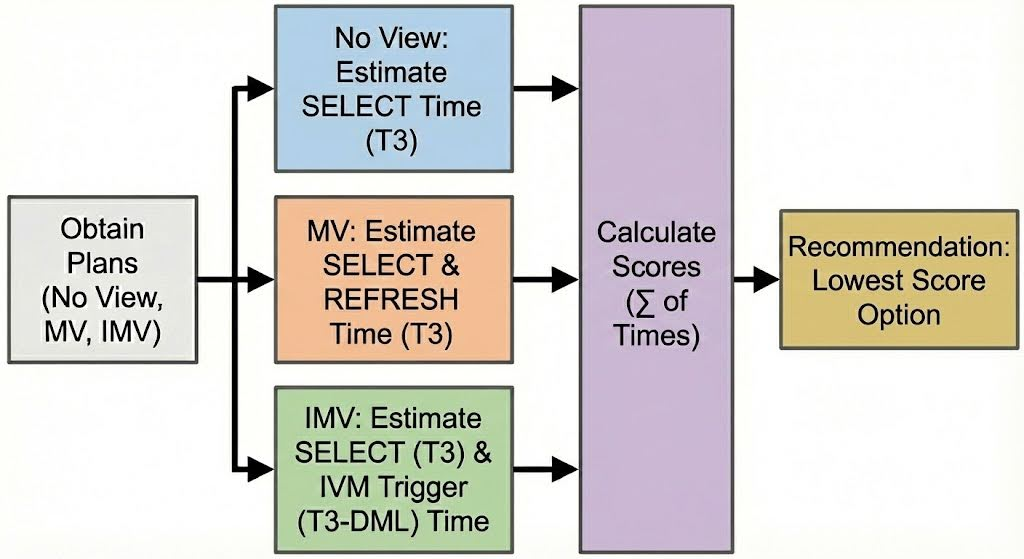
\includegraphics[width=0.8\textwidth]{view-advisor-flow.jpg}
    \caption{View Advisor Cost-Benefit Analysis Flow}
    \label{fig:view_advisor_flow}
\end{figure}

This setup allows the advisor to make informed decisions about view usage based on predicted performance impacts, leveraging the trained view refresh cost model to accurately estimate the overhead of \ac{IMV} maintenance.

\section{Summary}
\label{sec:methodology_summary}
This chapter outlined the comprehensive methodology for developing an \ac{ML}-based zero-shot view advisor. The process began with the careful curation of a labeled dataset through controlled execution of synthetic workloads, capturing both read and write performance metrics in the \ac{IMV} configuration. Feature extraction techniques were employed to transform \ac{QEP}s into numerical representations suitable for model training. The core of the methodology involved training a novel T3-style view refresh cost model to predict \ac{IMV} maintenance overhead. Finally, the trained model was integrated into a view advisor framework capable of recommending optimal view strategies based on cost-benefit analyses. This structured approach ensures that the advisor is grounded in empirical performance data and leverages advanced machine learning techniques to make informed recommendations.
% \chapter{Design}
\label{chap:design}
\IMRADlabel{methods} % Mechanismus um das Strukturierungsmodell IMRaD zu kennzeichnen

This chapter presents the design of the proposed ML-based view advisor. It first states the concrete objectives and system requirements derived from the problem statement, and then describes the proposed approach: system architecture, feature engineering, cost-model development and training, and the advisor integration and evaluation plan.

\section{Objectives}
\label{sec:requirements}
The primary objective of this thesis is to build a machine learning advisor that recommends the best view strategy for an arbitrary SQL workload: (i) materialized view (MV) with full recomputation, (ii) incrementally maintained materialized view (IMV), or (iii) no view. To achieve this objective the following requirements are identified:

\begin{enumerate}
    \item \textbf{Performance metrics.} Define clear, measurable metrics that capture both \emph{view maintenance cost} and \emph{query execution time} so that different strategies can be compared on the same basis.
    \item \textbf{Dataset curation.} Produce a labeled dataset of query execution times for reads and writes across the three view configurations (MV, IMV, no view). Each dataset entry must include the query, its QEP(s), and measured execution times under controlled experimental conditions.
    \item \textbf{Feature extraction.} Provide a pipeline-based feature extractor that maps QEPs into numerical feature vectors for both read and write queries.
    \item \textbf{Write cost model.} Design and train a decision-tree-based model (LightGBM) to predict per-tuple maintenance time for write pipelines; the read-cost model is assumed available.
    \item \textbf{Advisor logic.} Combine read- and write-cost predictions to estimate total workload time and produce a lowest-cost recommendation (MV / IMV / no view).
    \item \textbf{Evaluation.} Validate the advisor on unseen workloads and measure (a) prediction accuracy of the cost models, and (b) the advisor's success rate at selecting the true optimal strategy.
\end{enumerate}

\section{Proposed Approach}
\label{sec:proposed_approach}
To address the research questions posed in this thesis, we adopt a learning-based, workload-driven approach. The design is organized into four main phases: (1) system architecture, (2) featurization of SQL queries, (3) development and training of cost models, and (4) advisor integration and evaluation.

\subsection{System Architecture}
\label{sec:system_architecture}
The proposed system comprises three primary components (see Figure~\ref{fig:system}):

\begin{itemize}
    \item \textbf{Feature extractor.} Parses a query's Query Execution Plan (QEP) and decomposes it into a set of pipelines. For each pipeline the extractor builds a numerical feature vector that summarizes operator-level properties, pipeline flow statistics, and relevant schema/table statistics.
    \item \textbf{Cost models.} Two specialized models are used:
    \begin{itemize}
        \item \emph{Read cost model:} predicts the execution time of \texttt{SELECT} queries under each view configuration. A pre-existing read-cost model will be reused for this component.
        \item \emph{Write cost model:} predicts the execution time of write queries (\texttt{INSERT}, \texttt{UPDATE}, \texttt{DELETE}) with an emphasis on per-tuple maintenance cost for view maintenance pipelines.
    \end{itemize}
    \item \textbf{View advisor.} Given a workload (a sequence or distribution of SQL statements), the advisor queries the cost models for each statement under the three view scenarios, sums predicted pipeline costs to obtain per-statement and per-workload totals, and recommends the strategy with minimal predicted total workload time.
\end{itemize}

\subsection{Feature Engineering}
\label{sec:feature_engineering}
Feature engineering is split by query type (read vs.\ write) and follows a pipeline-centric decomposition.

\paragraph{Read queries}
For reads, we adopt the feature set and extraction procedures inspired by the T3 system \cite{rieger2025t3}. Features are derived from the QEP and include:
\begin{itemize}
    \item Operator-level attributes: operator type, estimated and actual output cardinalities, estimated cost, operator-specific metrics (e.g., join method).
    \item Table/column statistics: table size, column data types, histograms or distribution summaries where available.
    \item Pipeline-level aggregates: number of operators, depth of pipeline, estimated pipeline cost.
\end{itemize}
These features are designed to capture computational complexity and to enable the read-cost model to predict whether a view will accelerate the query.

\paragraph{Write queries}
For writes we use a similar pipeline-based representation but focus on tuple-centric and maintenance-relevant features:
\begin{itemize}
    \item Tuple-flow features: fraction/percentage of tuples from the pipeline start that reach particular operators (selectivity estimates).
    \item Operator-level features: operator cardinalities, output row width, estimated intermediate sizes.
    \item View-related features: number of joins and aggregations present in the view definition, and expected delta sizes that the maintenance pipeline must process.
    \item Physical costs: index lookup counts, number of affected partitions/pages where measurable.
\end{itemize}
Additionally, execution plans will be used to extract and treat distinct pipelines separately so the model can learn pipeline-specific per-tuple costs.

\subsection{Cost Model Development and Training}
\label{sec:cost_model}
The write cost model will be implemented as a LightGBM gradient-boosted decision-tree ensemble. The model training follows these principles:

\begin{itemize}
    \item \textbf{Training objective:} predict per-tuple processing time for a pipeline. The per-tuple formulation enables scaling predictions to arbitrary input cardinalities by multiplication with predicted/actual cardinalities at inference time.
    \item \textbf{Target transformation:} to stabilize training across a wide dynamic range of per-tuple times, the target per-tuple time \(t\) will be transformed via:
    \[
        t' = -\log(t).
    \]
    \item \textbf{Training data:} the dataset is curated by running workloads (mixes of reads and writes) under the three view configurations and recording per-pipeline execution times, cardinalities, and QEP-derived features. The write dataset will include reconstructed/extracted workloads (e.g., the reconstructed Amazon Redshift workload referenced in \nameref{Initial Results}).
    \item \textbf{Evaluation metrics:} model accuracy will be measured using metrics such as Mean Absolute Percentage Error (MAPE) and Q-Error on a held-out test set, and compared against baseline heuristics (e.g., simple cardinality-based rules).
    \item \textbf{Deployment optimization:} the trained LightGBM ensemble will be compiled to native code (or efficiently embedded) to enable fast inference during advisor operation.
\end{itemize}

\subsection{Advisor Integration and Evaluation}
\label{sec:integration_evaluation}
The advisor integrates the read- and write-cost models to recommend a view strategy for a workload. The per-workload decision flow is:

\begin{enumerate}
    \item For each statement in the workload, obtain its QEP in each scenario: MV, IMV, and no view.
    \item Decompose each QEP into pipelines and extract feature vectors via the feature extractor.
    \item Predict per-pipeline per-tuple time using the appropriate cost model (read or write) and scale by predicted/actual pipeline cardinalities to obtain pipeline times.
    \item Sum pipeline times to obtain per-statement predicted times for each scenario.
    \item Aggregate per-statement times across the workload to compute total predicted workload time for MV, IMV, and no view.
    \item Recommend the strategy with the minimum predicted total workload time.
\end{enumerate}

\paragraph{Evaluation plan}
End-to-end experiments will validate the advisor by executing a suite of test workloads on the target database. For each workload:
\begin{itemize}
    \item Measure the \emph{actual} total execution time under each strategy (MV, IMV, no view).
    \item Compare the advisor's recommendation against the empirically best strategy. The primary success metric is the advisor's accuracy: the percentage of workloads for which it selected the best-performing strategy.
    \item Report secondary metrics including the advisor's predicted vs.\ actual total times, model error statistics (MAPE, Q-Error), and sensitivity analyses across workload mixes (read-heavy vs.\ write-heavy).
\end{itemize}

The next chapter describes implementation details and the experimental setup used to collect the dataset and run the evaluation.

% \chapter{Implementation}
\label{chap:implementation}

\section{Implementation Overview}
\label{sec:implementationOverview}

The implementation will realize the design above. Key implementation decisions described in the objectives include:

\begin{itemize}
    \item Using LightGBM for the write-cost decision-tree ensemble and compiling the resulting model for fast inference.
    \item Reusing the existing read-cost model and its feature extraction pipeline.
    \item Instrumenting the database/testing infrastructure to record per-statement execution times and execution plans across the three view configurations (no view, \ac{MV}, \ac{IMV}) to build the training dataset.
    \item Implementing an advisor component that consumes predicted read/write costs and applies the decision logic to produce a recommendation.
\end{itemize}

Further implementation details (choice of database system, workload generator parameters, exact instrumentation methods, and integration scripts) will be documented in Chapter~\ref{chap:implementation} as they are finalized and implemented.

\chapter{Evaluation}
\label{chap:evaluation}
\IMRADlabel{results} % Mechanismus um das Strukturierungsmodell IMRaD zu kennzeichnen

To evaluate the performance and usefulness of the proposed \ac{ML}-based view advisor, we conduct experiments on two key components: (1) the view refresh cost model, which predicts the maintenance overhead of \acp{IMV}, and (2) the view advisor itself, which recommends optimal view configurations for a given workload. This chapter presents the experimental setup, evaluation metrics, results, and analysis for both components.

\section{Experimental Setup}
\label{sec:experimentalSetup}

This section describes the experimental environment, datasets, and procedures used to evaluate the view refresh cost model and the view advisor.

\subsection{Hardware and Software Environment}
\label{sec:hardware_setup}

All experiments were conducted on a dedicated server to ensure consistent and reproducible results. The hardware specifications are detailed in Table~\ref{tab:hardware_specs} in Appendix~\ref{sec:hardware_specs}. The database system used for evaluation is PostgreSQL 16 with the \texttt{pg\_ivm} extension enabled for \ac{IMV} support.

\subsection{Evaluation Dataset}
\label{sec:eval_dataset}

For evaluation, we use the IMDB database, which was deliberately excluded from the training data to test the zero-shot generalization capabilities of our models. The IMDB database contains information about movies, actors, directors, and related metadata, providing a diverse set of tables and relationships suitable for view evaluation.

The evaluation workload consists of a set of \texttt{SELECT} and \ac{DML} queries derived from the Amazon Redshift workload \cite{gupta2015amazon}, filtered to those applicable to the IMDB schema. This represents a realistic workload for testing the view advisor's effectiveness.

\subsection{Candidate View Definitions}
\label{sec:view_definitions}

We curated a set of 12 candidate view definitions specifically designed for the IMDB database. While we acknowledge that 12 views is a small sample size for classification, these views represent common query patterns involving joins across multiple tables such as \texttt{title}, \texttt{cast\_info}, \texttt{movie\_companies}, and \texttt{name}. The complete SQL definitions for these views are provided in Appendix~\ref{sec:views}.

The candidate views vary in complexity:
\begin{itemize}
    \item \textbf{Simple views:} Two-table joins with basic filtering (e.g., Views 1, 2, 5, 7)
    \item \textbf{Complex views:} Three-table joins with multiple predicates (e.g., Views 3, 8, 9)
    \item \textbf{High-selectivity views:} Views with restrictive filter conditions (e.g., Views 4, 11)
\end{itemize}

The sequence of operations in the workload for each view query is illustrated in Figure~\ref{fig:workload_sequence}.
\begin{figure}[h!]
    \centering
    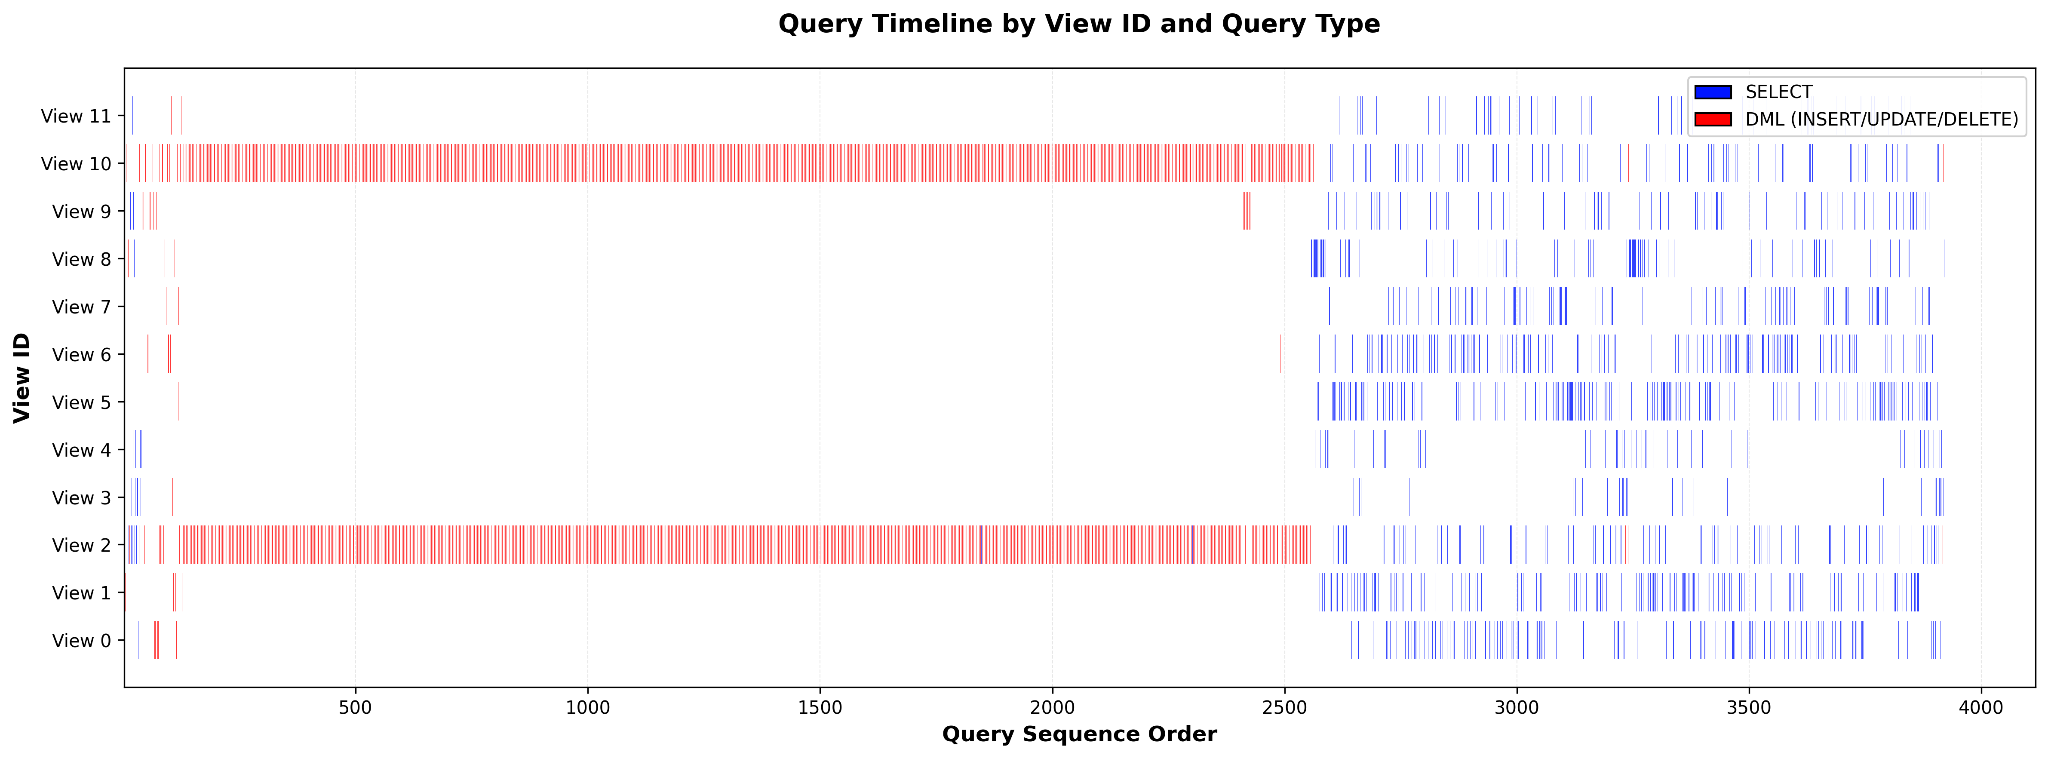
\includegraphics[width=0.8\textwidth]{IMDB-sequence.png}
    \caption{Workload Sequence for Each View Query}
    \label{fig:workload_sequence}
\end{figure}

\subsection{Query Rewriting}
\label{sec:query_rewriting}

To evaluate the benefit of views on read queries, we employ query rewriting techniques. For each \texttt{SELECT} query in the workload, we attempt to rewrite it to utilize one of the candidate views where applicable. The rewriting process identifies queries whose base tables and predicates match a subset of a candidate view's definition, allowing the query to be answered directly from the view instead of the base tables.

\subsection{Workload Generation Parameters}
\label{sec:workload_gen_params}

The workload generation parameters used for creating the training dataset are summarized in Table~\ref{tab:workload_params} in Appendix~\ref{sec:workload_parameters}. These parameters control the diversity and complexity of the generated queries, ensuring broad coverage of different query patterns.

\section{Evaluation of the View Refresh Cost Model}
\label{sec:eval_cost_model}

The first component we evaluate is the T3-style view refresh cost model, which predicts the execution time of \ac{IMV} maintenance triggers.

\subsection{Feature Importance}
\label{sec:feature_importance}

To understand the decision-making process of the learned view refresh cost model, we analyzed the feature importance scores generated by LightGBM (specifically the 'Gain' metric, which measures the improvement in accuracy brought by a feature to the branches it is on). Figure~\ref{fig:feature_importance} illustrates the top five most influential features.

\begin{figure}[h!]
    \centering
    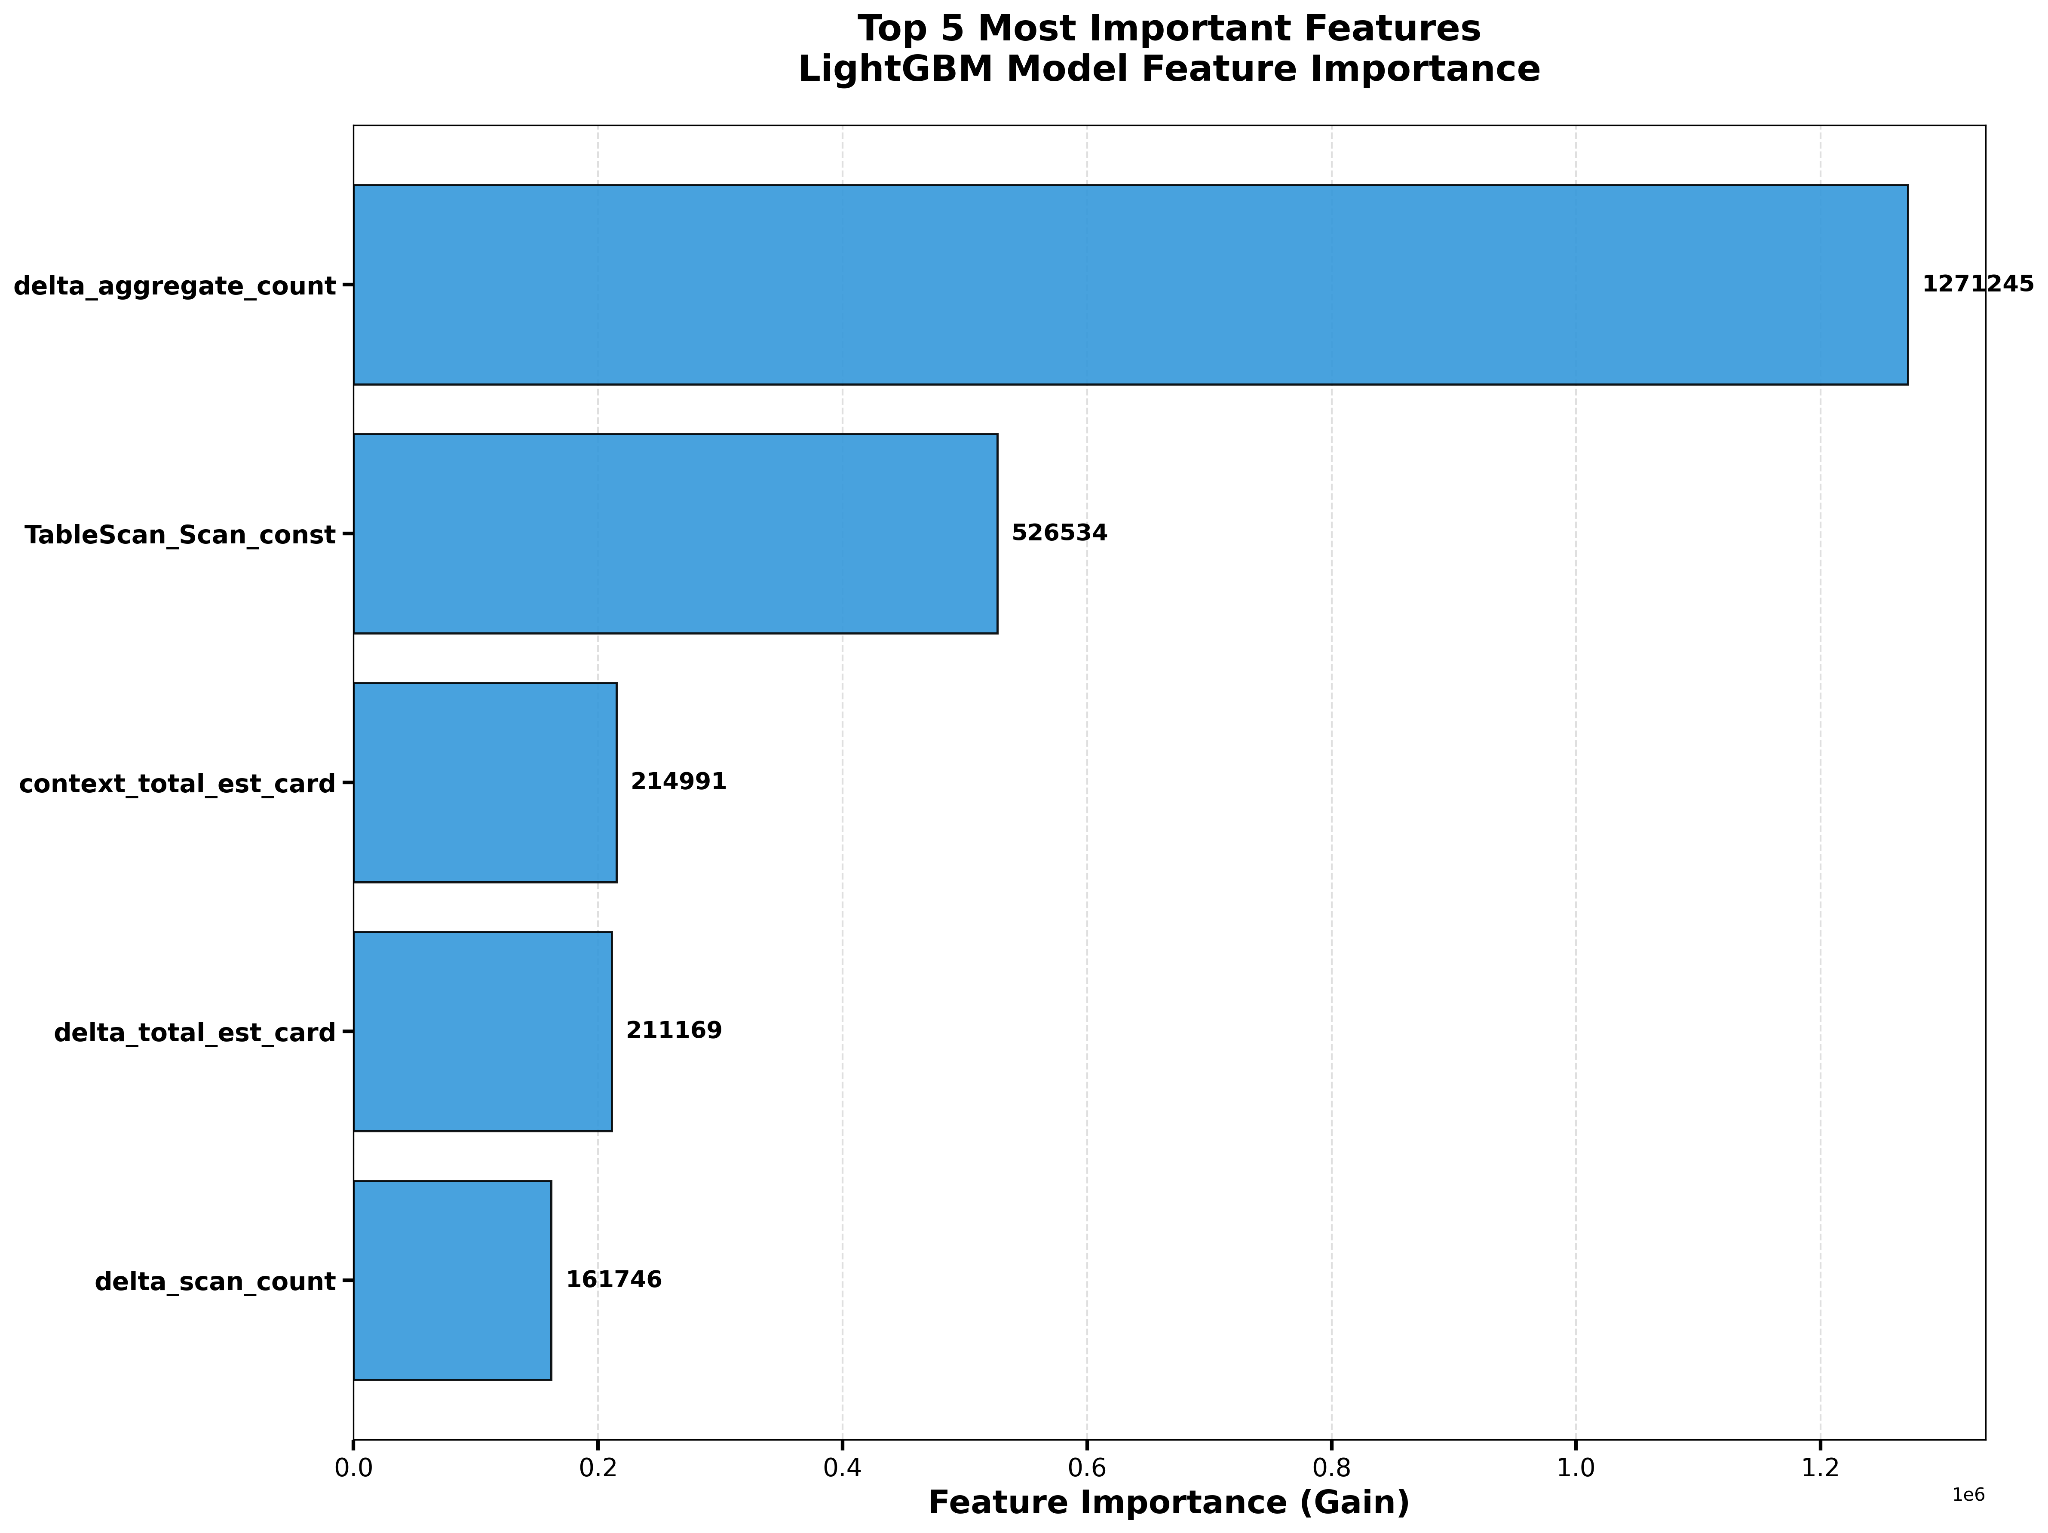
\includegraphics[width=0.7\textwidth]{feature_importance.png}
    \caption{Top 5 Feature Importances for the View Refresh Cost Model}
    \label{fig:feature_importance}
\end{figure}

The results validate our hypothesis that accurate IVM cost estimation requires a composite view of both the maintenance operation and the static view context.

\begin{itemize}
    \item \textbf{Dominance of Maintenance Complexity}: The single most important feature, \texttt{delta\_aggregate\_count}, indicates that the presence of aggregation operations within the trigger logic is the primary driver of maintenance cost. This aligns with the theoretical understanding that maintaining aggregates (e.g., updating SUM or COUNT) requires stateful logic that is computationally heavier than simple projections.
    \item \textbf{Validation of Context Features}: Crucially, \texttt{context\_total\_est\_card} appears as the third most important feature. This confirms that the model relies heavily on the static size of the view (a "Context Feature" introduced in Section~\ref{sec:feature_extraction}) to scale its predictions. Without this feature, the model would lack the necessary context to distinguish between updates on small versus large datasets, leading to the zero-shot failures observed in early experiments.
    \item \textbf{Role of Interaction Features}: The presence of \texttt{TableScan\_Scan\_const} and \texttt{delta\_scan\_count} highlights that the I/O overhead of locating tuples--both in the base table and the view--remains a critical cost factor.
\end{itemize}

\subsection{Evaluation Procedure}
\label{sec:cost_model_procedure}

To evaluate the view refresh cost model, we follow these steps:
\begin{enumerate}
    \item \textbf{Create \acp{IMV}:} For each candidate view definition in Appendix~\ref{sec:views}, we create an \ac{IMV} using the \texttt{pg\_ivm} extension.
    \item \textbf{Execute \ac{DML} workload:} For each \ac{DML} statement in the IMDB workload that affects the base tables of the created views, we executed the statement and capture the actual execution time of the \ac{IVM} triggers that maintain the view.
    \item \textbf{Extract \ac{QEP}s:} For each executed \ac{DML} statement, we extract the \ac{QEP} of the associated \ac{IVM} trigger. We excluded all \ac{QEP}s that have zero cardinality, as they do not contribute to view maintenance.
    \item \textbf{Featurize \ac{QEP}s:} The \ac{QEP}s are featurized according to the methodology described in Section~\ref{sec:feature_extraction}, extracting delta features, context features, and interaction features.
    \item \textbf{Predict execution times:} Using the trained view refresh cost model, we predict the execution time for each \ac{DML} statement.
    \item \textbf{Compare predictions:} We compare the predicted execution times with the actual measured times using standard regression metrics.
\end{enumerate}

\subsection{Evaluation Metrics}
\label{sec:cost_model_metrics}

We evaluate the view refresh cost model using the following metrics:

\begin{itemize}
    \item \textbf{Mean Squared Error (MSE):} Measures the average squared difference between predicted and actual values:
    \[
    \text{MSE} = \frac{1}{n} \sum_{i=1}^{n} (y_i - \hat{y}_i)^2
    \]
    
    \item \textbf{Mean Absolute Percentage Error (MAPE):} Measures the average percentage error:
    \[
    \text{MAPE} = \frac{100\%}{n} \sum_{i=1}^{n} \left| \frac{y_i - \hat{y}_i}{y_i} \right|
    \]
    
    \item \textbf{Q-Error:} A multiplicative error metric commonly used in database cost estimation:
    \[
    \text{Q-Error} = \max\left(\frac{y_i}{\hat{y}_i}, \frac{\hat{y}_i}{y_i}\right)
    \]
    We report the median and 95th percentile Q-Error.
\end{itemize}

\subsection{Results}
\label{sec:cost_model_results}

Table~\ref{tab:cost_model_results} presents the evaluation results of the view refresh cost model on the IMDB dataset.

\begin{table}[h!]
    \centering
    \caption{View Refresh Cost Model Evaluation Results}
    \label{tab:cost_model_results}
    \begin{tabular}{lr}
        \toprule
        \textbf{Metric} & \textbf{Value} \\
        \midrule
        MSE & 103.13 \\
        MAPE & 59.54\% \\
        Median Q-Error & 3.66 \\
        95th Percentile Q-Error & 3.72 \\
        Spearman Rank & 0.08 \\
        \bottomrule
    \end{tabular}
\end{table}

% TODO: Fill in actual results and add analysis

\subsection{Analysis}
\label{sec:cost_model_analysis}

The evaluation results on the unseen IMDB workload demonstrate the zero-shot generalization capabilities of the proposed model, as well as the inherent challenges of cross-database transfer.

The most significant finding is the consistency of the error. While the Median Q-Error is 3.66, the 95th percentile Q-Error is remarkably close at 3.72. This narrow distribution indicates that the error is systematic rather than random. The model consistently over-predicts the maintenance cost by a factor of roughly 3.7×. Due to this bias, we propose that a few-shot calibration step (by running a few probe queries on the target database and observing the hardware scaling factor) could significantly improve absolute accuracy in future work.

We attribute this bias to the specific characteristics of the training data. The training set included the \texttt{tournament} dataset, which contained extreme outliers (max runtime ≈29 seconds) and high-cardinality tables. The model likely learned to associate high-cardinality context features (like those found in IMDB) with the severe performance penalties observed in tournament. However, the IMDB test environment proved to be more performant than the worst-case scenarios in the training set, leading to a consistent over-estimation of costs.

Despite the scaling bias, the stability of the Q-Error across the workload suggests that the Context Features successfully captured the relative complexity of the views. If the model had failed to learn the structural differences between views (e.g., distinguishing a 2-table join from a 5-table join), we would expect a much wider variance in Q-Error (e.g., a P95 significantly higher than the median). The tight clustering of error metrics confirms that the model correctly ranks the relative expensiveness of operations, even if the absolute magnitude is shifted.

The Spearman Rank correlation (0.08) remains low, indicating that while the model captures the coarse-grained "macro" costs (distinguishing between light and heavy workloads via Context features), it struggles to rank fine-grained differences between queries hitting the same view. This limitation is expected given that the static context features dominate the feature importance (Section \ref{sec:feature_importance}), making queries on the same view appear similar to the model.

It is also worth noting that, while at the first glance the MAPE of 59.54\% looks relatively high, this is influenced by the presence of low-latency updates in the workload, where small absolute errors translate to large percentage errors. For example, a prediction error of 0.5 seconds on a 1-second operation results in a 50\% MAPE contribution. In contrast, the Q-Error metric is more robust to such cases, as it treats over- and under-estimations symmetrically.

\section{Evaluation of the View Advisor}
\label{sec:eval_view_advisor}

Having validated the accuracy of the underlying cost models, we now evaluate the end-to-end performance of the View Advisor. The primary goal is to determine whether the advisor can correctly select the optimal view strategy (no view, \ac{MV}, or \ac{IMV}) for a given workload, even when transferred zero-shot to the unseen IMDB database.

\subsection{Evaluation Procedure}
\label{sec:view_advisor_procedure}

To evaluate the view advisor, we follow these steps:
\begin{enumerate}
    \item \textbf{Create views:} For each candidate view definition, we create both an \ac{MV} and an \ac{IMV}. The database is reset between configurations to ensure isolation.
    \item \textbf{Rewrite workload:} The read queries in the workload are rewritten to use the view definitions where applicable, as described in Section~\ref{sec:query_rewriting}.
    \item \textbf{Estimate \ac{QEP}s:} For each configuration (no view, \ac{MV}, \ac{IMV}), we obtain the estimated \ac{QEP}s for all queries in the workload.
    \item \textbf{Compute scores:} For each view definition, we group its associated read and \ac{DML} queries and compute the total score:
    \[
    \text{Score} = \sum \text{(predicted read time)} + \sum \text{(predicted refresh time)}
    \]
    For the ``no view'' configuration, the predicted refresh time is zero.
    \item \textbf{Select optimal configuration:} For each view definition, we select the configuration (no view, \ac{MV}, or \ac{IMV}) with the lowest score.
    \item \textbf{Execute and measure:} To determine the ground-truth optimal configuration, we executed the workload under all three configurations and measure actual execution times.
\end{enumerate}

\paragraph{Note on \ac{IMV} Trigger Plan Estimation.}
During evaluation, we discovered that PostgreSQL's \texttt{EXPLAIN} command cannot generate estimated plans for \ac{IVM} trigger execution. This is because triggers are executed implicitly as part of \ac{DML} operations, and their plans are not accessible through standard plan inspection interfaces. To address this limitation, we executed the \ac{DML} queries with \ac{IVM} triggers enabled and capture the actual execution times. We then use the T3 \ac{DML} cost model to predict the \ac{IVM} trigger time and compare it to the actual measured time.

\subsection{Impact on Total Workload Runtime}
\label{sec:workload_runtime}

Since the ultimate goal of the view advisor is ranking and risk avoidance rather than pure classification, the metric that matters most is the total time saved across the entire workload. Figure~\ref{fig:total_runtime} illustrates the aggregate impact of the advisor's recommendations.

\begin{figure}[h!]
    \centering
    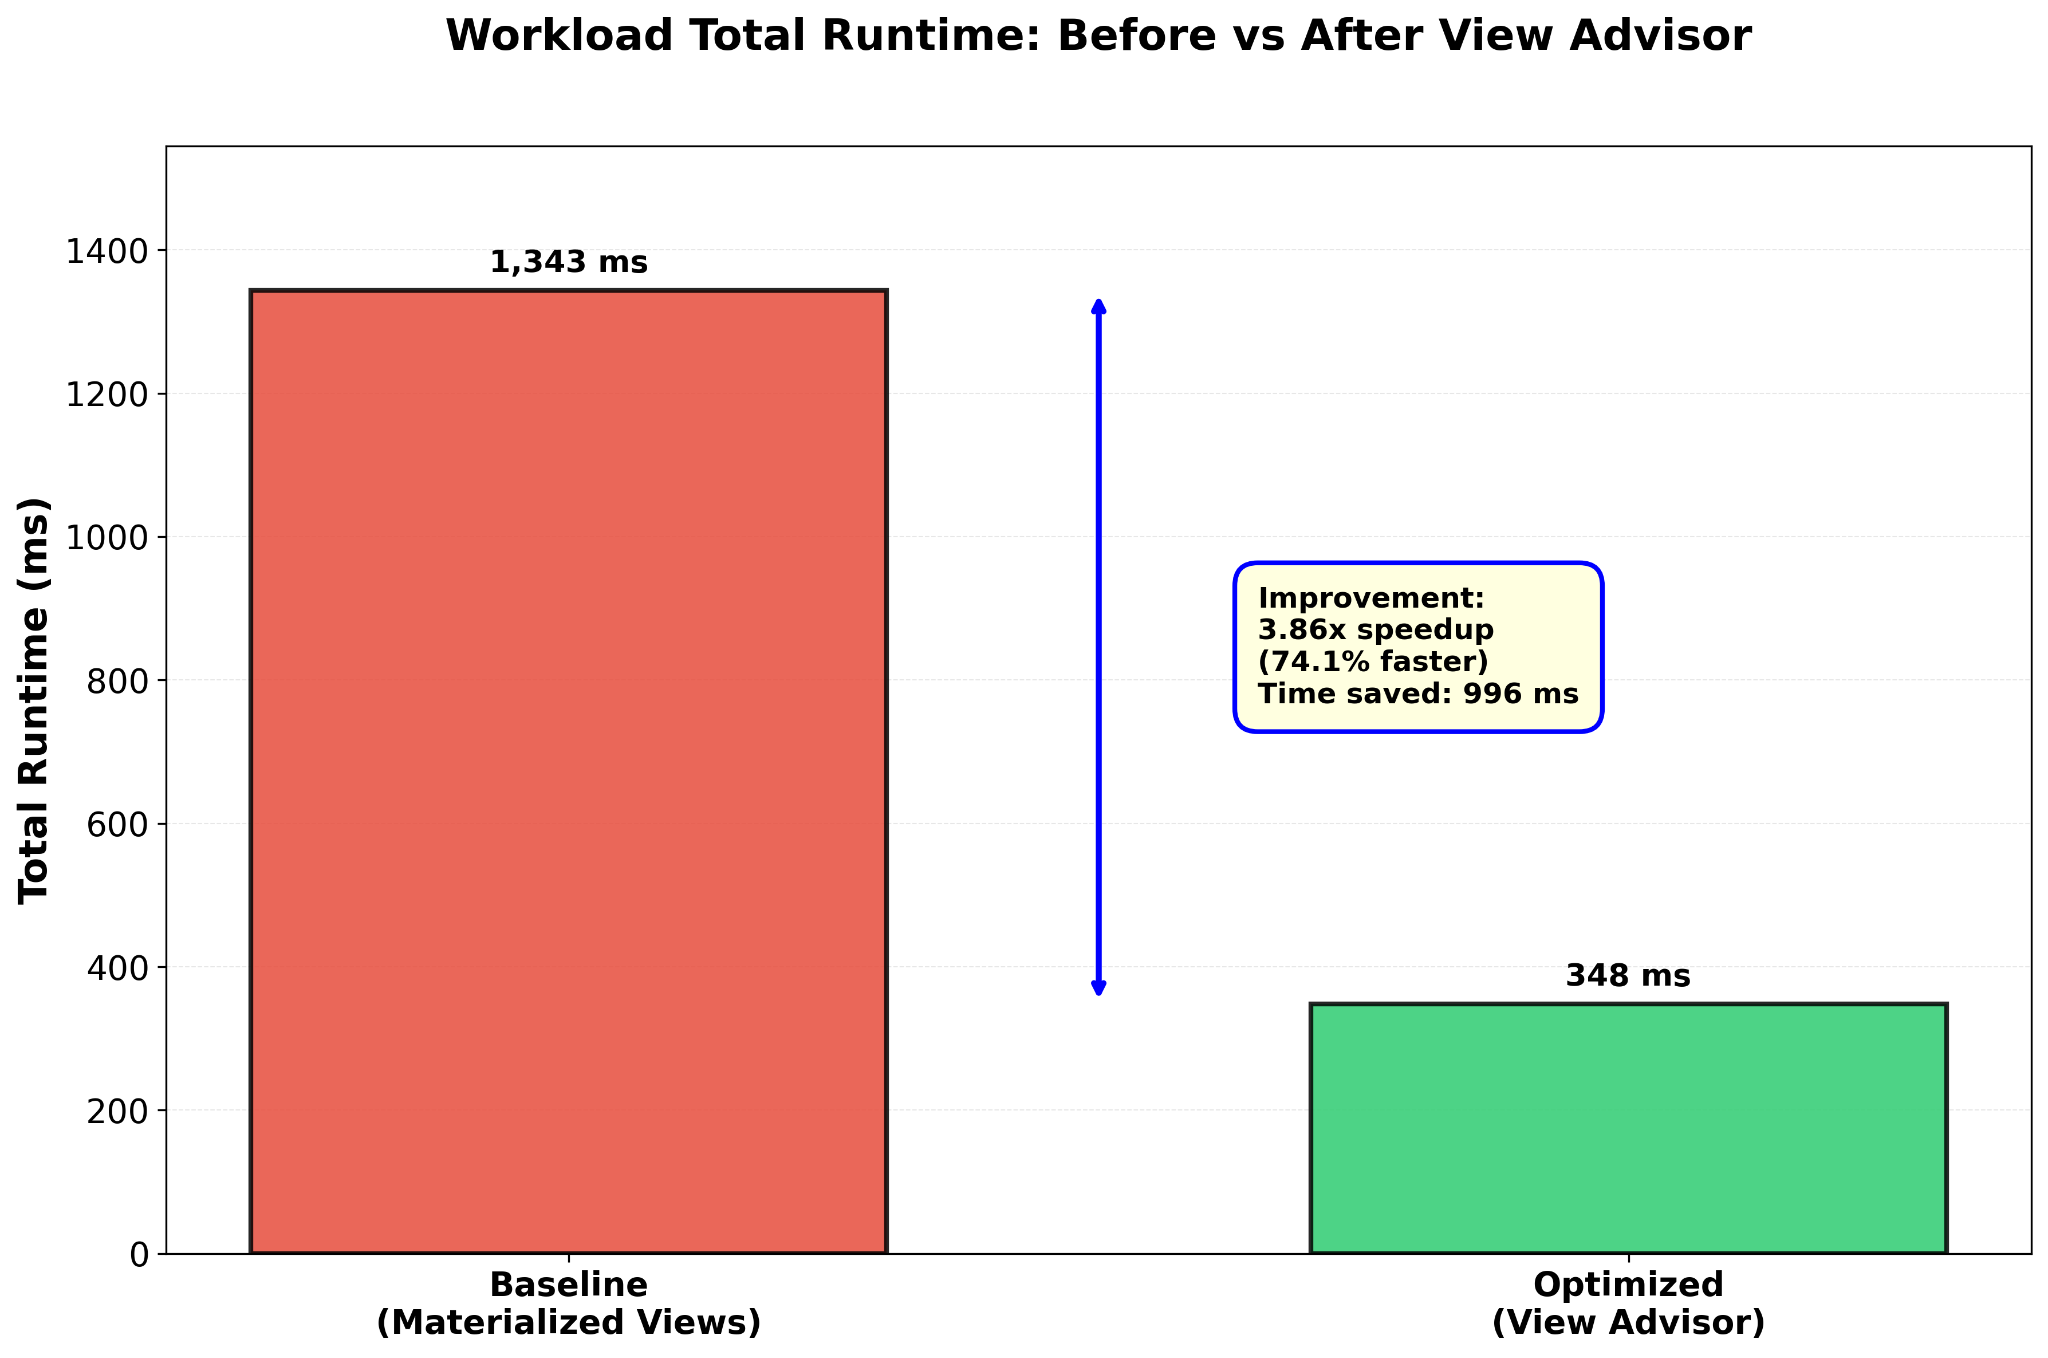
\includegraphics[width=0.9\textwidth]{view-advisor-total-workload-runtime-speedup.png}
    \caption{Total Workload Runtime: Baseline vs. Advisor Recommendations}
    \label{fig:total_runtime}
\end{figure}

\begin{itemize}
    \item \textbf{Baseline Runtime:} 1,343 ms (using standard \acp{MV} for all views).
    \item \textbf{Optimized Runtime:} 348 ms (using the Advisor's recommended mix of strategies).
    \item \textbf{Speedup:} The advisor achieved a \textbf{3.86$\times$ speedup} (74.1\% reduction in runtime).
\end{itemize}

This result confirms that the advisor successfully identifies the high-impact optimization opportunities. It correctly navigated the trade-off space to filter out expensive \ac{MV} maintenance where appropriate (switching to No View mode or \ac{IMV}), resulting in a substantial net performance gain.

\subsection{Decision Accuracy and Tolerance}
\label{sec:decision_accuracy}

To assess the quality of the advisor's recommendations, we compared its predicted optimal strategy against the ground-truth optimal strategy (determined by executing all configurations).

\paragraph{Strict Accuracy.}
Under strict evaluation, the advisor achieves an accuracy of 41.67\% (5 out of 12 views). In these cases, the advisor's top choice exactly matched the ground truth. While this may appear modest at first glance, it is important to recognize that view selection is fundamentally a ranking problem, not a classification problem. The absolute difference in cost between strategies can vary dramatically across views.

\paragraph{Relaxed Accuracy (Tolerance).}
In many database tuning scenarios, "near-optimal" decisions are acceptable. For example, if No View mode costs 100ms and \ac{IMV} costs 105ms, choosing \ac{IMV} is technically incorrect but practically negligible. We define a tolerance threshold $\tau$: a prediction is considered correct if the chosen strategy's cost is within $\tau\%$ of the true optimal cost:
\[
\frac{|T_{\text{recommended}} - T_{\text{optimal}}|}{T_{\text{optimal}}} \leq \tau
\]

Figure~\ref{fig:accuracy_vs_tolerance} illustrates how recommendation accuracy varies with tolerance.

\begin{figure}[h!]
    \centering
    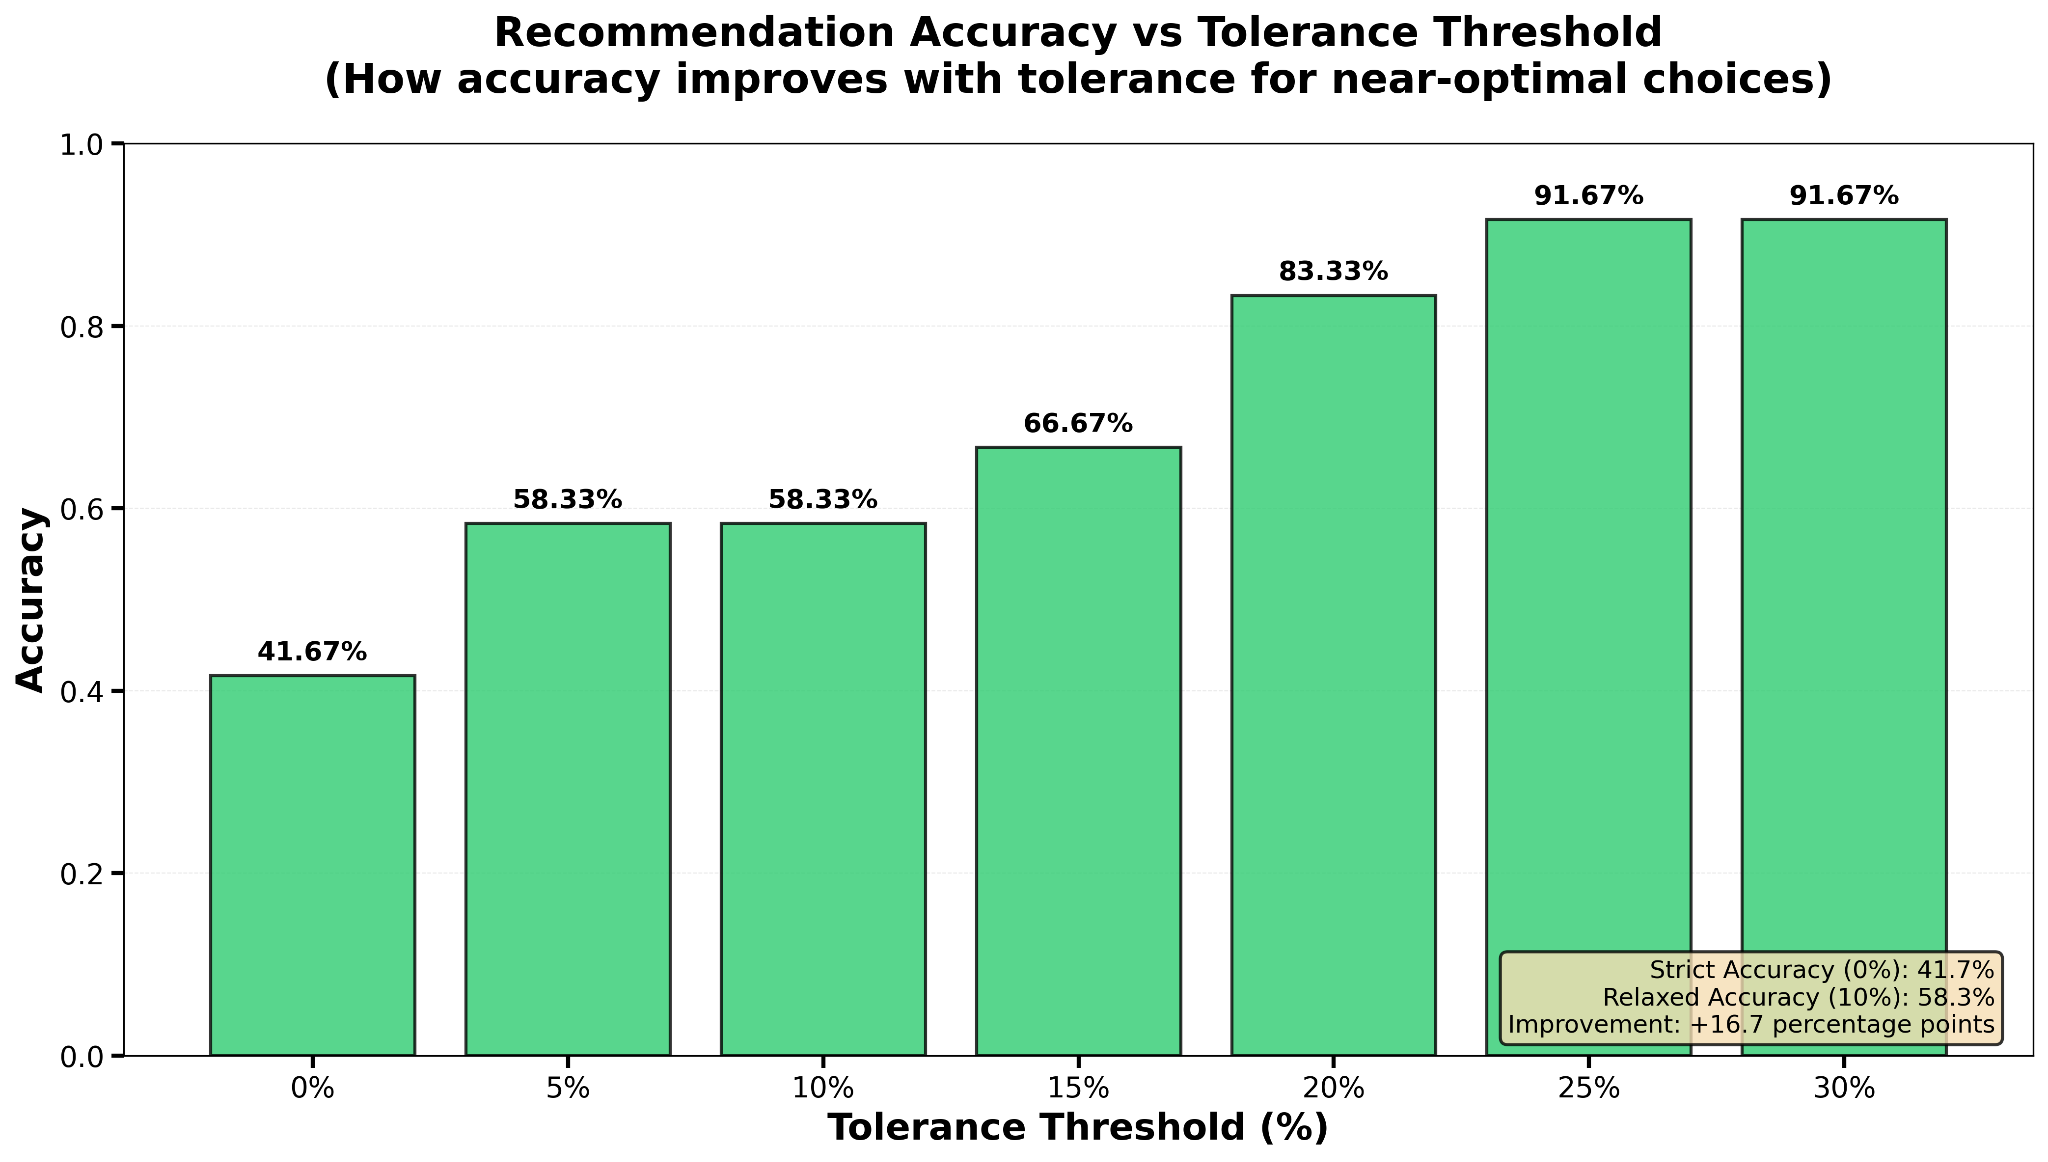
\includegraphics[width=0.8\textwidth]{view-advisor-recommendation-accuracy-vs-tolerance-threshold.png}
    \caption{Recommendation Accuracy as a Function of Tolerance Threshold}
    \label{fig:accuracy_vs_tolerance}
\end{figure}

From the figure, we observe the following:
\begin{itemize}
    \item At a modest 5\% tolerance, accuracy increases to 58.33\%.
    \item At a 25\% tolerance, accuracy reaches 91.67\%, meaning the advisor avoids catastrophic decisions in nearly all cases.
    \item This demonstrates that while the advisor sometimes misses the absolute best strategy in "close call" scenarios, it consistently identifies competitive strategies that are within the same performance tier.
\end{itemize}

\subsection{Error Analysis: Confusion Matrix}
\label{sec:confusion_matrix}

Figure~\ref{fig:confusion_matrix} provides a detailed breakdown of the advisor's decision errors through a confusion matrix.

\begin{figure}[h!]
    \centering
    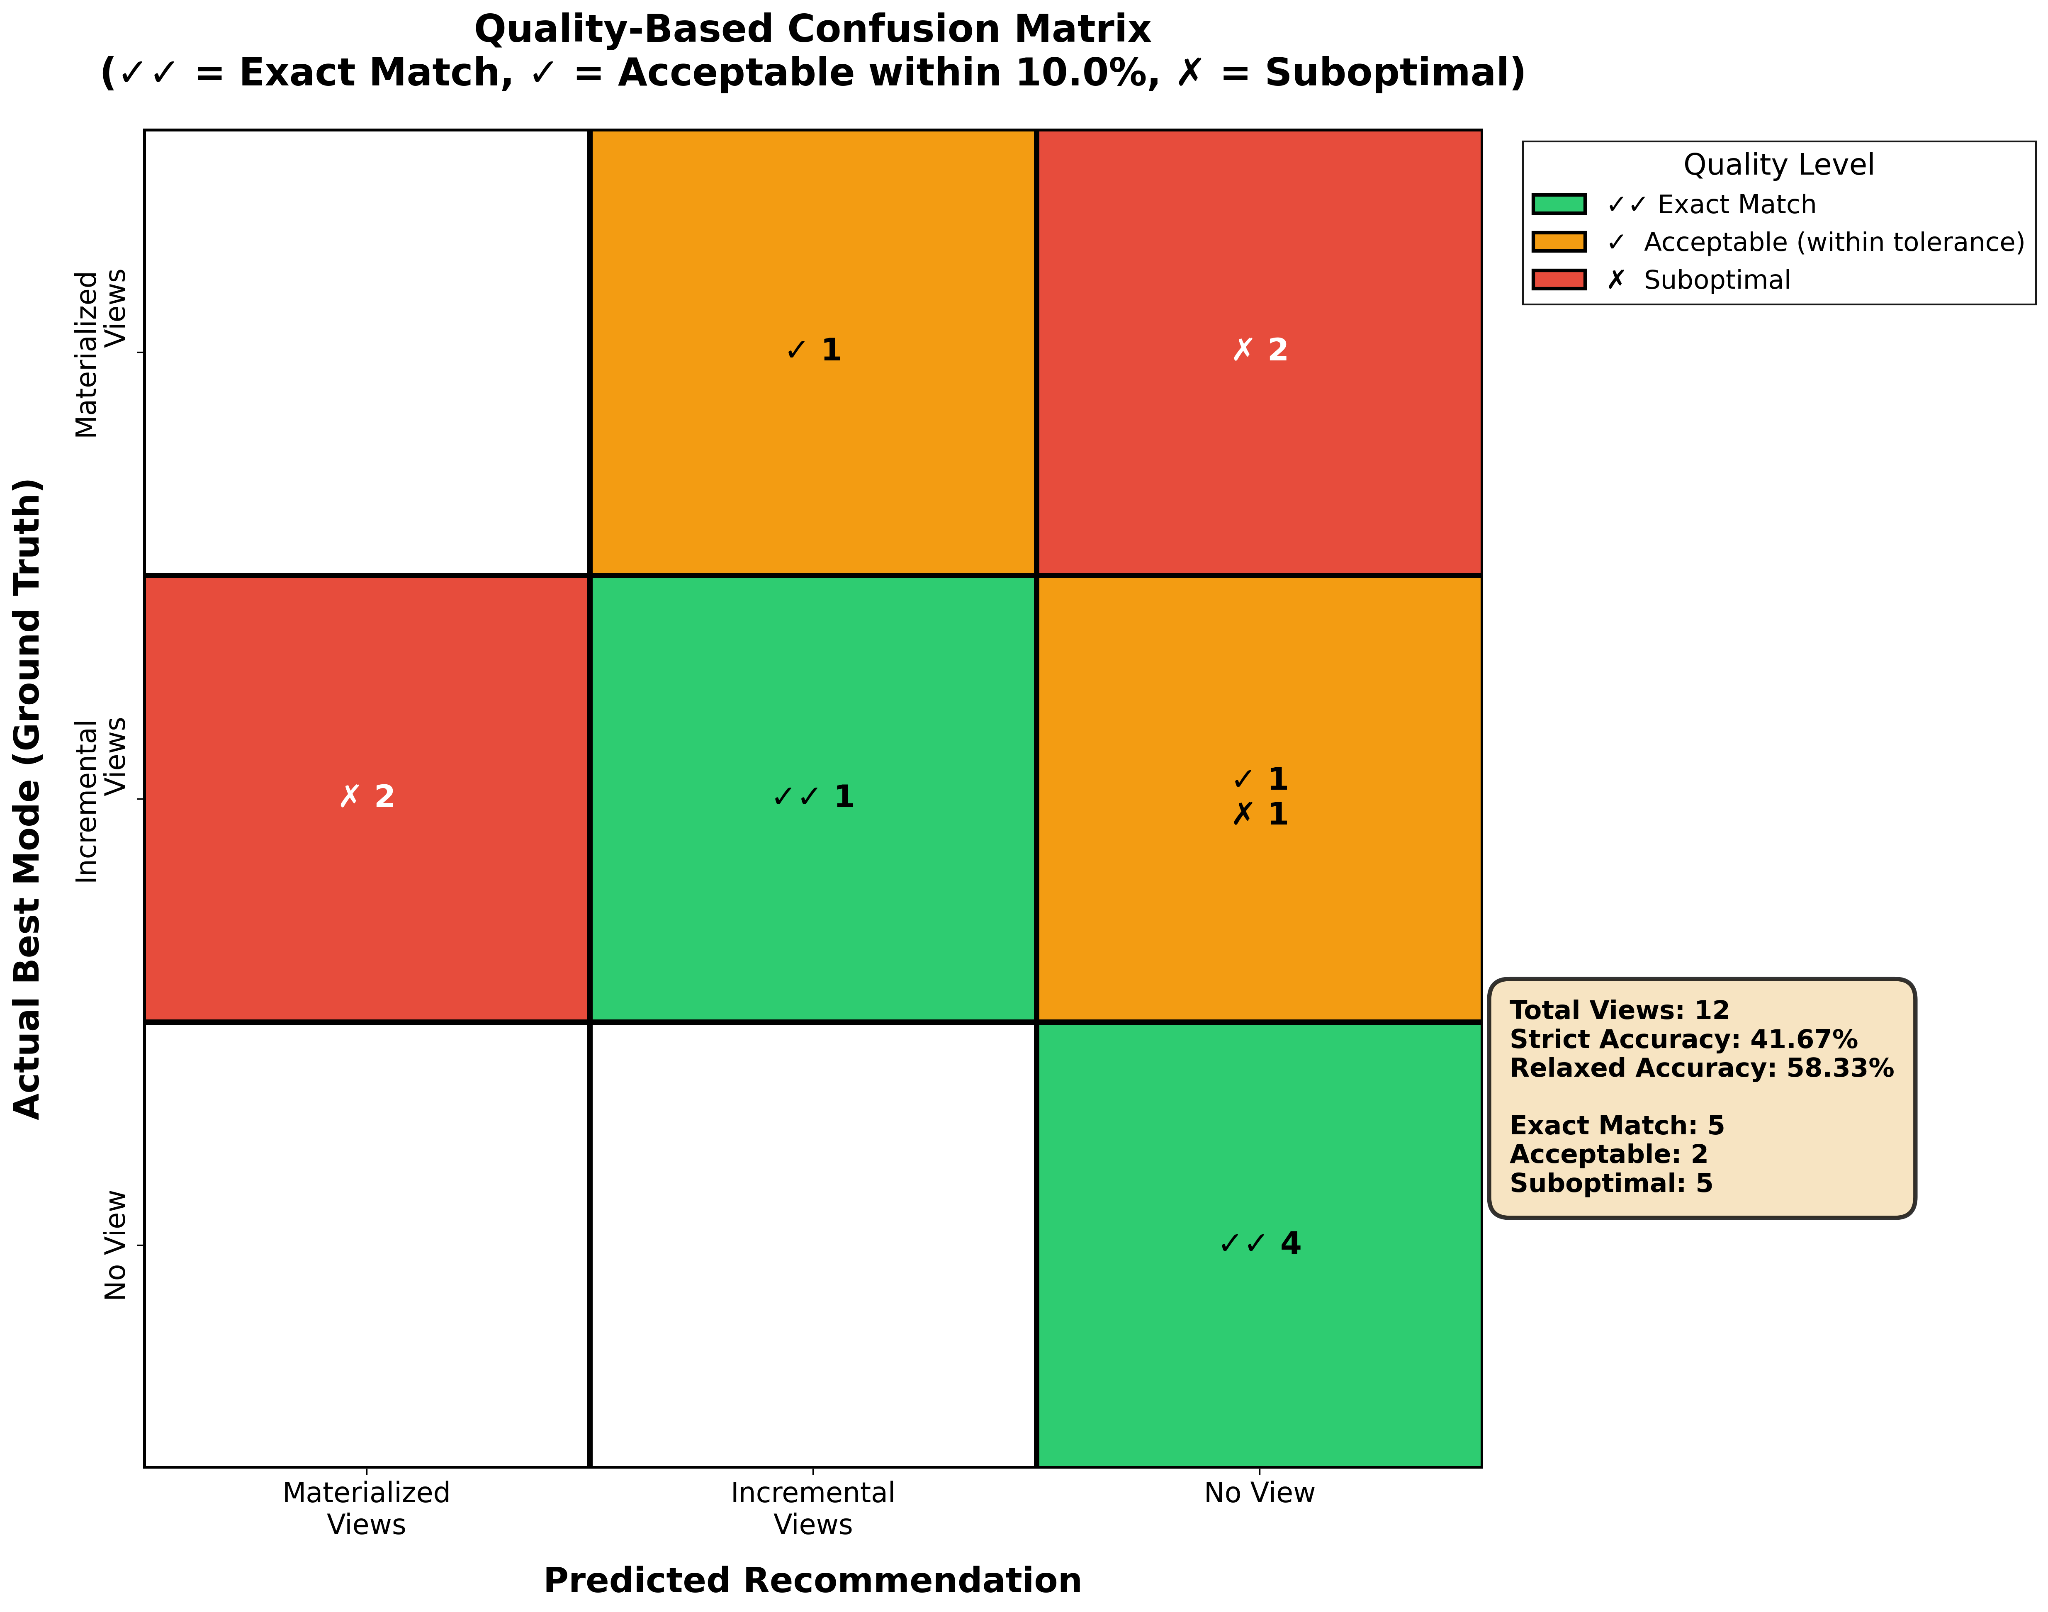
\includegraphics[width=0.8\textwidth]{view-advisor-confusion-matrix.png}
    \caption{Confusion Matrix for View Advisor Recommendations}
    \label{fig:confusion_matrix}
\end{figure}

The confusion matrix reveals a specific pattern of misclassification:

\paragraph{Conservative Bias.}
The most common error type is predicting No View mode when the true optimal was \ac{IMV} or \ac{MV} modes (False Negatives). This indicates that the advisor exhibits risk-averse behaviour, as it requires a strong signal of benefit to recommend creating a view. In production environments, this is often a desirable property, as it avoids the overhead of creating and maintaining unnecessary views that provide marginal benefits.

\paragraph{The "Close Call" Problem.}
Many of the errors labeled as "Suboptimal ($\times$)" occur when the costs of two strategies are extremely close. For instance, the advisor may predict that No View and \ac{IMV} modes have nearly identical costs (within 10\%), but minor estimation noise causes the ranking to be inverted. While technically incorrect, the utility difference is marginal, and either choice would yield satisfactory performance.

\paragraph{Absence of Catastrophic Errors.}
Notably, there are no cases where the advisor recommended an expensive \ac{MV} mode when No View mode was clearly superior (or vice versa with large margins). This confirms that the advisor successfully avoids the most damaging misconfigurations.

\subsection{Per-View Speedup Analysis}
\label{sec:per_view_speedup}

To understand which views contributed most to the overall speedup, we examined the per-view performance improvements. Figure~\ref{fig:per_view_speedup} shows the speedup achieved for each candidate view.

\begin{figure}[h!]
    \centering
    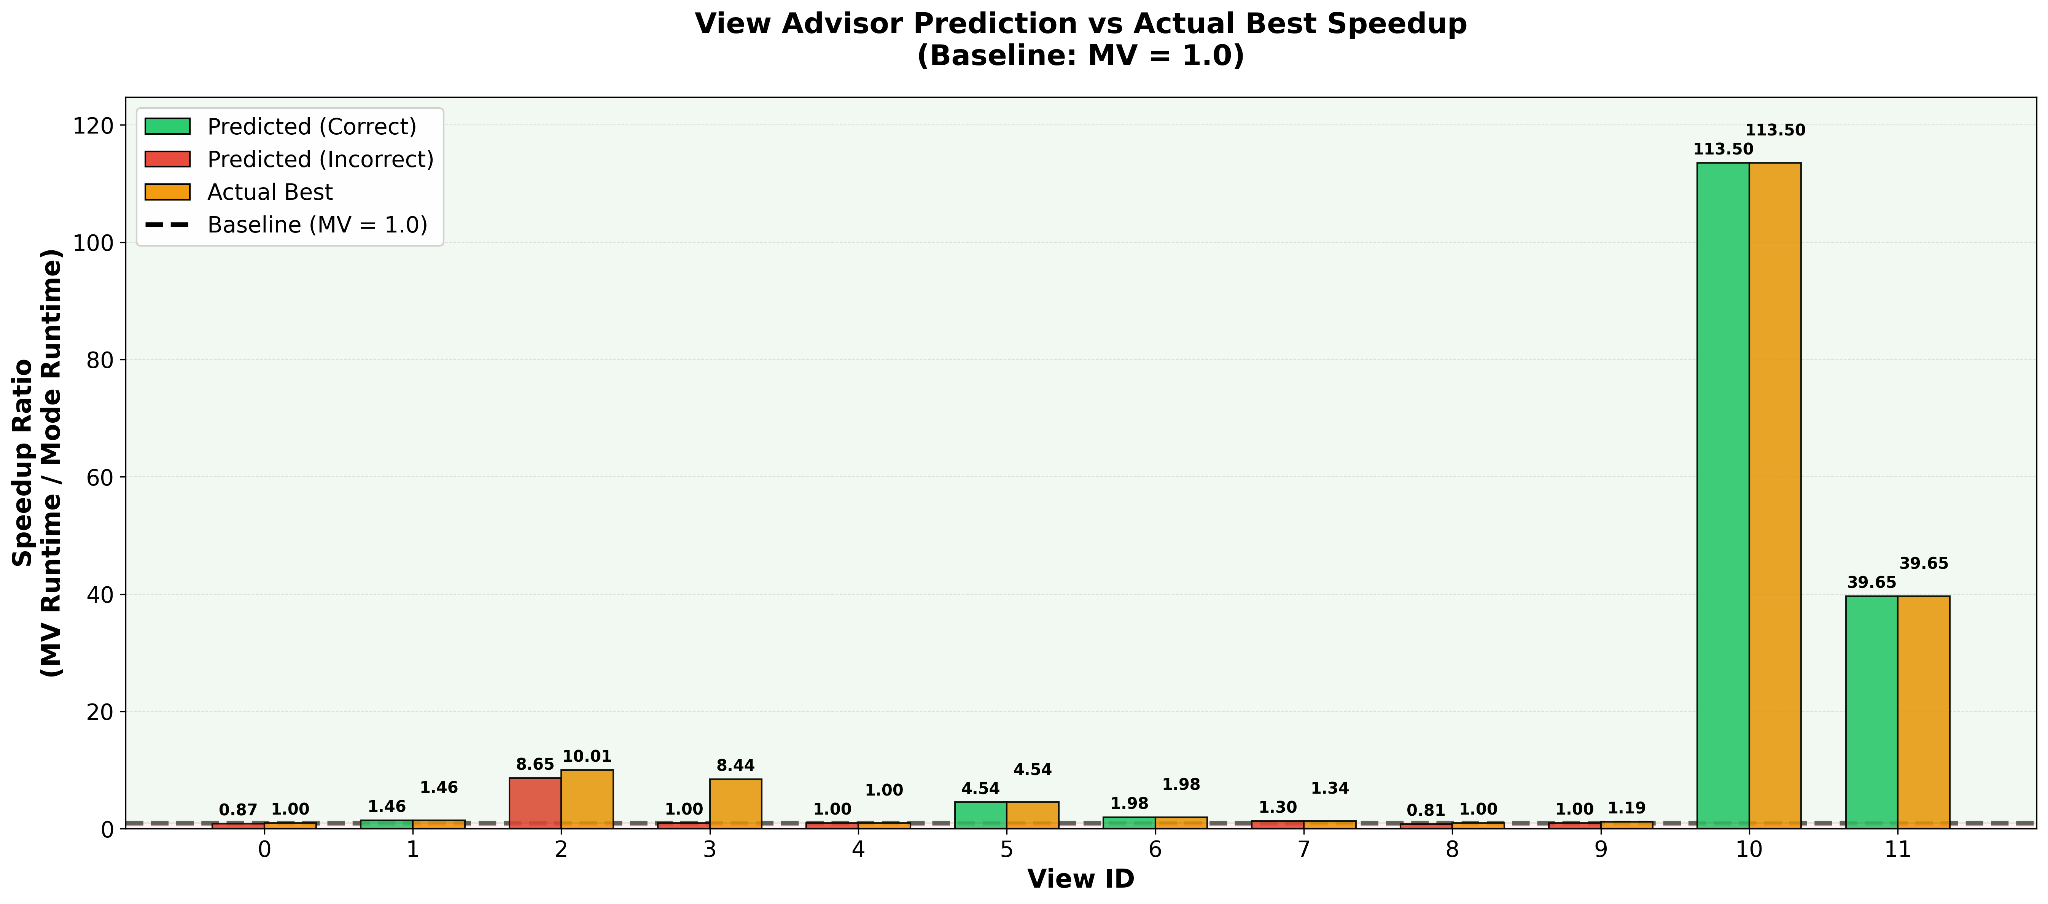
\includegraphics[width=0.9\textwidth]{view-advisor-per-view-prediction-label.png}
    \caption{Speedup per View Definition (Advisor vs. Baseline)}
    \label{fig:per_view_speedup}
\end{figure}

Key observations:
\begin{itemize}
    \item \textbf{High-impact views:} Views 10 and 11 achieved massive speedups ($>$10$\times$) by switching from expensive \ac{MV} maintenance to more efficient strategies. These views had high write-to-read ratios, making full recomputation prohibitively expensive. This massive speedup alone accounts for a significant portion of the overall workload improvement. This indicates that, instead of perfectly ranking all configurations--including the configurations with incremental speedups--, the advisor effectively identifies the views where materialization provides the largest marginal benefit.
    
    \item \textbf{Marginal-benefit views:} For Views 2, 4, and 6, the advisor correctly identified that materialization provided minimal benefit and recommended No View mode, avoiding unnecessary overhead.
    
    \item \textbf{Conservative decisions:} In a few cases (e.g., View 3), the advisor chose a suboptimal but safe strategy, resulting in near-unity speedup (neither gain nor loss).
\end{itemize}

\subsection{Analysis}
\label{sec:view_advisor_analysis}

The evaluation demonstrates that the view advisor is effective at making high-level strategic decisions about view usage, even when individual cost predictions contain systematic bias.

\paragraph{Why Low Strict Accuracy Does Not Imply Poor Performance.}
The 41.67\% strict accuracy might suggest poor decision-making at first glance. However, when contextualized with the tolerance analysis and total runtime results, a different picture emerges:
\begin{itemize}
    \item The advisor achieves 91.67\% accuracy at 25\% tolerance, indicating it rarely makes disastrous choices.
    \item The 3.86$\times$ speedup demonstrates that the advisor correctly identifies the views where materialization provides the largest marginal benefit.
    \item In database tuning, the goal is to maximize aggregate performance, not to perfectly rank every configuration. The advisor succeeds at this macro-level optimization.
\end{itemize}

\paragraph{The Role of Conservative Bias.}
The confusion matrix reveals that the advisor errs on the side of caution, preferring No View mode when uncertain. This is a feature, not a bug:
\begin{itemize}
    \item Creating and maintaining unnecessary views incurs storage and update overhead.
    \item In production systems, false positives (recommending a bad view) are more costly than false negatives (missing a beneficial view).
    \item The conservative bias aligns with industry best practices, where views are created only when there is clear evidence of benefit.
\end{itemize}

\paragraph{Generalization Across Workload Types.}
The advisor successfully handles diverse workload characteristics:
\begin{itemize}
    \item \textbf{Read-heavy workloads:} For views with high read-to-write ratios, the advisor correctly recommends \ac{IMV} or \ac{MV} modes, as the maintenance overhead is amortized over many read operations.
    \item \textbf{Write-heavy workloads:} For views with frequent updates, the advisor appropriately recommends No View mode or selectively uses \ac{IMV} modes when incremental maintenance is efficient.
    \item \textbf{Mixed workloads:} The advisor's cost-benefit analysis effectively balances competing objectives, selecting configurations that minimize total execution time.
\end{itemize}

The systematic over-estimation of maintenance costs essentially acts as a high confidence threshold, as the advisor only recommends a materialized view mode when the read-side benefit is overwhelming, ensuring that resources are not wasted on marginal candidates.

\section{Discussion}
\label{sec:discussion}

\subsection{Limitations}
\label{sec:limitations}

Despite the promising results, several limitations should be noted regarding the current approach:

\begin{itemize}
    \item \textbf{Zero-Shot Extrapolation limits:} Tree-based models are inherently limited in their ability to extrapolate to feature values outside their training range. As observed in the IMDB evaluation, when the target database contains tables significantly larger than those in the training set (e.g., millions vs. hundreds of thousands of rows), the model tends to predict the maximum cost learned during training or systematic bias, rather than scaling linearly.
    
    \item \textbf{\ac{IMV} trigger plan estimation:} PostgreSQL does not currently support `EXPLAIN` for internal \ac{IVM} triggers without execution. Consequently, the advisor must execute the \ac{DML} statements on a sample or staging environment to capture the trigger plans for feature extraction, which introduces a runtime overhead to the recommendation process.
    
    \item \textbf{View complexity:} The current evaluation is limited to views with up to 3 joins. More complex views involving window functions, nested subqueries, or `DISTINCT` clauses may have non-linear maintenance costs that are not fully captured by the current feature set.
    
    \item \textbf{Concurrent workloads:} The evaluation assumes serial execution of queries. In practice, concurrent read/write workloads may experience lock contention on the materialized view or the \ac{IVM} delta tables, a dynamic overhead that the static cost model does not currently predict.
\end{itemize}

\subsection{Threats to Validity}
\label{sec:threats}

\begin{itemize}
    \item \textbf{Internal validity:} To control for noise, all experiments were conducted on dedicated hardware with a warm cache. However, the use of a 10\% sample for plan capture in the advisor introduces a sampling bias, where fixed overheads (planning, connection) may dominate execution time compared to full-scale runs.
    
    \item \textbf{External validity:} The evaluation focuses on the \texttt{pg\_ivm} extension for PostgreSQL. While the methodology (context features + total time prediction) is generalizable, the specific feature importance (e.g., the dominance of specific scan types) is likely implementation-specific. Additionally, the IMDB dataset, while a standard benchmark, represents only one point in the schema design space (snowflake-like schema with heavy skew).
    
    \item \textbf{Construct validity:} We utilized standard regression metrics (Q-Error, MAPE) and classification metrics (Accuracy, F1). However, the ultimate ground truth for an advisor is the end-to-end workload runtime, which we prioritize in our final analysis over pure prediction accuracy.
\end{itemize}

\section{Summary}
\label{sec:evaluation_summary}

This chapter presented a comprehensive evaluation of the \ac{ML}-based View Advisor and its underlying write-cost model. The results support the following conclusions:

\begin{enumerate}
    \item \textbf{Feasibility of Learned IVM Cost Estimation:} We demonstrated that a tree-based model using \textit{Context Features} (static view definition) and \textit{Interaction Ratios} can successfully distinguish between low-cost and high-cost maintenance operations. While zero-shot transfer introduces systematic bias due to hardware and scale differences, the model successfully preserves the relative rank of costs, achieving a median Q-Error of $3.66\times$ on the unseen IMDB workload.
    
    \item \textbf{Robust Decision Making:} Despite the challenges of zero-shot cost estimation, the View Advisor demonstrates high utility. While the strict decision accuracy is $41.67\%$, the relaxed accuracy at a $25\%$ tolerance threshold reaches $91.67\%$. This indicates that even when the advisor misclassifies a view, it selects a strategy that is competitively close to the optimal performance.
    
    \item \textbf{Significant Workload Acceleration:} The ultimate validation of the system is the aggregate impact on query processing. The advisor's recommendations resulted in a \textbf{$3.86\times$ speedup} (reducing total cost from 1,343 ms to 348 ms) compared to a baseline of fully materialized views.
\end{enumerate}

These findings confirm that an automated, learned approach to view selection is not only viable but capable of delivering substantial performance gains by effectively navigating the trade-off between read acceleration and incremental maintenance overhead.

\chapter{Conclusion and Future Work}
\label{chap:conclusion_futurework}

This work addressed the challenge of automating physical design decisions for \ac{IVM} in PostgreSQL. While \ac{IVM} offers a compelling trade-off between read latency and data freshness, its write-side overhead is non-trivial and highly workload-dependent. We proposed, implemented, and evaluated a Machine Learning-based advisor capable of navigating this trade-off to recommend the optimal view strategy---No View, Materialized View, or Incremental View---for arbitrary SQL workloads.

\section{Conclusion}
\label{sec:conclusion}

The primary contributions of this work were the design of the advisor framework, the development of a novel write-cost estimation model that addresses the specific challenges of incremental maintenance, and the empirical evaluation of their zero-shot capabilities.

We successfully designed a view advisor that treats view selection as a cost-benefit optimization problem. By integrating read-cost estimates with our novel write-cost predictions, the advisor constructs a holistic view of the workload's performance profile. Crucially, our research highlights that accurate IVM advising requires observing internal trigger logic which is not exposed by standard \texttt{EXPLAIN} commands. Consequently, we designed the advisor to operate as a "What-If" analysis tool, leveraging a staging or sampling phase to capture the necessary trigger plans. The system demonstrates that learned models can effectively trade off read acceleration against write penalties, provided this planning phase is accommodated.

A core technical contribution of this thesis is the adaptation of the \ac{T3} cost modeling approach for \ac{IVM} maintenance. We demonstrated that standard tuple-centric prediction targets fail for maintenance workloads due to the presence of fixed overheads and non-linear scaling. To overcome this, we introduced a model that predicts per-pipeline \textit{View Refresh Time}, augmented by a composite feature engineering strategy. This strategy combines \textit{Delta Features} (from trigger execution plans) with \textit{Static Context Features} (from view definitions). This architecture allows the model to capture the interaction between update volume and view size, an important factor for zero-shot transfer.

The evaluation on the held-out IMDB benchmark demonstrated the practical utility of the approach despite the challenges of zero-shot transfer.
\begin{itemize}
    \item \textbf{Workload Acceleration:} The ultimate validation of the system is the aggregate impact on query processing. The advisor's recommendations resulted in a \textbf{$3.86\times$ speedup} for the total workload runtime compared to a baseline of fully materialized views. This confirms that the advisor successfully identifies and filters out scenarios where the cost of \ac{IMV} maintenance outweighs the read benefits.
    \item \textbf{Robust Decision Making:} While strict classification accuracy was limited to $41.67\%$ due to estimation noise in "close call" scenarios, the advisor achieved a \textbf{$91.67\%$ relaxed accuracy} within a 25\% tolerance threshold. This indicates that the system is highly effective at risk avoidance, consistently selecting strategies that are either optimal or competitively close to optimal.
    \item \textbf{Generalization and Calibration:} The write-cost model achieved a median Q-Error of $3.66\times$ on the unseen IMDB workload. The consistency between the median and $95^{th}$ percentile error ($3.72\times$) suggests that while the model successfully ranks relative costs, it suffers from a systematic scaling bias due to lack of input features on hardware overhead. This finding points toward the necessity of a "few-shot" calibration step in future work to align the model's absolute predictions with the target environment.
\end{itemize}

\section{Future Work}
\label{sec:future_work}

While this work establishes a strong foundation for learned \ac{IVM} advisors, several avenues for future research remain to enhance the system's accuracy and practicality.

\paragraph{Trigger Plan Estimation without Execution}
Currently, extracting features for the write-cost model requires executing \ac{DML} statements on a staging environment to capture the \ac{IVM} trigger plans. This introduces significant overhead. Future work should investigate modifying the PostgreSQL engine or the \texttt{pg\_ivm} extension to expose "Estimated Trigger Plans" via the standard \texttt{EXPLAIN} command. This would allow the advisor to operate in a purely hypothetical mode, drastically reducing the time required to generate recommendations.

\paragraph{Advanced Plan Representation}
The current model uses a flat, aggregate feature representation of the query plan. While effective for estimating the order of magnitude, the low Spearman rank correlation (0.08) indicates a limitation in fine-grained ranking. Future research could explore Graph Neural Networks (GNNs) or Tree-LSTM architectures to encode the full structure of the trigger plans. These deep learning approaches may better capture subtle operator interactions that tree-based models miss, potentially improving the ranking accuracy in zero-shot scenarios.

\paragraph{Concurrency and Lock Contention}
The current cost model assumes serial execution and focuses on resource consumption (CPU/IO). However, in high-throughput transactional workloads, the primary bottleneck for \ac{IMV} is often lock contention on the view or the delta tables. Developing a "Concurrency-Aware" cost model that predicts lock wait times based on write frequency and transaction isolation levels would be a critical step toward deploying \ac{IMV} advisors in operational OLTP environments.

\paragraph{Automatic Calibration}
Our evaluation revealed a systematic bias when transferring models between disparate hardware environments (e.g., "Tournament" training data vs. IMDB test environment). Future iterations of the advisor could implement an online learning module that runs a small sample of "probe" queries on the target database (Few-Shot Learning). By comparing the predicted vs. actual costs of these probes, the system could automatically calibrate its scaling factors, reducing the systematic prediction error and improving decision accuracy without full retraining.

		
\printbibliography


\begin{appendices}

\addtocontents{toc}{\protect\setcounter{tocdepth}{1}}
\makeatletter
\addtocontents{toc}{%
  \begingroup
  \let\protect\l@chapter\protect\l@section
  \let\protect\l@section\protect\l@subsection
}

\chapter{Experiment Parameters}
\label{appendix:experiment_parameters}
The experiments conducted in the \nameref{chap:evaluation} Chapter were executed with the following DPI parameters. Note, an \textit{x} indicates the parameter has been varied for the experiment.

\section{Workload Generation Parameters}
\label{sec:workload_parameters}
The main workload used for training and evaluation, referred to as \texttt{workload\_200k\_imv}, was generated using the parameters listed in Table~\ref{tab:workload_params}.

\begin{table}[h!]
  \centering
  \caption{Parameters for \texttt{workload\_200k\_imv}}
  \label{tab:workload_params}
  \begin{tabular}{ll}
    \toprule
      \textbf{Parameter} & \textbf{Value} \\ 
    \midrule
      \texttt{num\_queries} & 200,000 \\
      \texttt{min\_no\_joins} & 0 \\
      \texttt{max\_no\_joins} & 3 \\
      \texttt{min\_no\_predicates} & 1 \\
      \texttt{max\_no\_predicates} & 3 \\
      \texttt{min\_no\_aggregates} & 1 \\
      \texttt{max\_no\_aggregates} & 3 \\
      \texttt{max\_no\_group\_by} & 0 \\
      \texttt{max\_cols\_per\_agg} & 2 \\
      \texttt{seed} & 1 \\ 
    \bottomrule
  \end{tabular}
\end{table}


\section{Hardware Specifications}
\label{sec:hardware_specs}
All workloads were executed on a machine with the type \texttt{c8220}. The key hardware and software specifications for this node are detailed in Table~\ref{tab:hardware_specs}.

\begin{table}[h!]
  \centering
  \caption{Hardware and OS Specifications}
  \label{tab:hardware_specs}
  \begin{tabular}{ll}
    \toprule
      \textbf{Component} & \textbf{Specification} \\ 
    \midrule
      Machine Type & c8220 \\
      Architecture & x86\_64 \\
      Processor & Intel E5-2660v2 \\
      CPU Speed & 2200 MHz \\
      CPU Sockets & 2 \\
      Cores per Socket & 10 \\
      Threads per Core & 2 \\
      Total Logical Cores & 40 (2 \texttimes{} 10 \texttimes{} 2) \\
      Total Memory & 262144 MB (256 GB) \\
      Operating System & Ubuntu 22.04 (UBUNTU22-64-STD) \\
    \bottomrule
  \end{tabular}
\end{table}

% ADD the view queries used for IMDB workload evaluation
\section{IMDB Candidate View Definitions}
\label{sec:appendix_queries}

The following SQL queries were used to define the views for the evaluation of the view advisor.

\begin{lstlisting}[caption={Query 1: Join on Title and AKA Title with phonetic filtering}]
SELECT "title"."id" AS "title_id", "aka_title"."id" AS "aka_title_id", "title"."kind_id", "aka_title"."movie_id", "title"."production_year", "aka_title"."title" AS "aka_title", "aka_title"."note" AS "aka_note" 
FROM "title" 
JOIN "aka_title" ON "title"."id" = "aka_title"."movie_id" 
WHERE "aka_title"."movie_id" = "title"."id" 
AND "aka_title"."phonetic_code" BETWEEN 'A1652' AND 'Z6564' 
AND "title"."title" BETWEEN '(#1.10964)' AND 'üç';
\end{lstlisting}

\begin{lstlisting}[caption={Query 2: Movie Companies and Types}]
SELECT "movie_companies"."id", "movie_companies"."company_id", "movie_companies"."movie_id", "movie_companies"."note", "company_type"."kind" 
FROM "movie_companies" 
JOIN "company_type" ON "movie_companies"."company_type_id" = "company_type"."id" 
WHERE "company_type"."kind" BETWEEN 'distributors' AND 'special effects companies' 
AND "movie_companies"."note" BETWEEN '(1911) (USA) (theatrical)' AND 'co-production)';
\end{lstlisting}

\begin{lstlisting}[caption={Query 3: Title, Info Index, and Keywords}]
SELECT "title"."id", "title"."season_nr", "title"."episode_of_id", "title"."phonetic_code", "title"."episode_nr", "title"."production_year", "movie_info_idx"."info", "movie_keyword"."keyword_id" 
FROM "title" 
JOIN "movie_info_idx" ON "title"."id" = "movie_info_idx"."movie_id" 
JOIN "movie_keyword" ON "title"."id" = "movie_keyword"."movie_id" 
WHERE "title"."production_year" BETWEEN 1900 AND 2025;
\end{lstlisting}

\begin{lstlisting}[caption={Query 4: Movie Info and Title Metadata}]
SELECT "movie_info"."id" AS "movie_info_id", "movie_info"."movie_id", "movie_info"."info_type_id", "movie_info"."info", "movie_info"."note", "title"."id" AS "title_id", "title"."title", "title"."imdb_index", "title"."kind_id", "title"."production_year", "title"."imdb_id", "title"."phonetic_code", "title"."episode_of_id", "title"."season_nr", "title"."episode_nr", "title"."series_years", "title"."md5sum" 
FROM "movie_info" 
JOIN "title" ON "movie_info"."movie_id" = "title"."id" 
WHERE "title"."md5sum" BETWEEN '0296d2b20235be36849d015e34d80f2c' AND 'fffffec1b13bc6af69f56864884364e4' 
AND "movie_info"."note" BETWEEN 'ôtre k''ôtre' AND 'ôtre k''ôtre';
\end{lstlisting}

\begin{lstlisting}[caption={Query 5: Cast Info ordering}]
SELECT "title"."id" AS "title_id", "cast_info"."person_id", "cast_info"."person_role_id", "cast_info"."nr_order" 
FROM "title" 
JOIN "cast_info" ON "cast_info"."movie_id" = "title"."id" 
WHERE "cast_info"."nr_order" BETWEEN 0 AND 100;
\end{lstlisting}

\begin{lstlisting}[caption={Query 6: Person Info and Name}]
SELECT "name"."id", "name"."name", "name"."imdb_index", "name"."gender", "name"."name_pcode_nf", "name"."name_pcode_cf", "name"."surname_pcode", "name"."md5sum", "person_info"."info", "person_info"."note", "person_info"."info_type_id" 
FROM "name" 
JOIN "person_info" ON "name"."id" = "person_info"."person_id" 
WHERE "person_info"."info_type_id" BETWEEN 15 AND 39;
\end{lstlisting}

\begin{lstlisting}[caption={Query 7: Linked Movies}]
SELECT "movie_link"."id", "movie_link"."movie_id", "movie_link"."linked_movie_id", "movie_link"."link_type_id", "link_type"."link" AS "link_type" 
FROM "movie_link" 
JOIN "link_type" ON "movie_link"."link_type_id" = "link_type"."id" 
WHERE "movie_link"."linked_movie_id" BETWEEN 11104 AND 2524994;
\end{lstlisting}

\begin{lstlisting}[caption={Query 8: Name, AKA Name, and Person Info Join}]
SELECT "name"."id" AS "name_id", "aka_name"."id" AS "aka_name_id", "person_info"."id" AS "person_info_id", "aka_name"."person_id", "person_info"."person_id" AS "person_info_person_id", "person_info"."info_type_id", "name"."gender" 
FROM "name" 
JOIN "aka_name" ON "name"."id" = "aka_name"."person_id" 
JOIN "person_info" ON "name"."id" = "person_info"."person_id";
\end{lstlisting}

\begin{lstlisting}[caption={Query 9: Completed Cast Status}]
SELECT "title"."id" AS "title_id", "complete_cast"."id" AS "complete_cast_id", "comp_cast_type"."id" AS "comp_cast_type_id", "complete_cast"."movie_id", "complete_cast"."subject_id", "complete_cast"."status_id" 
FROM "title" 
JOIN "complete_cast" ON "title"."id" = "complete_cast"."movie_id" 
JOIN "comp_cast_type" ON "complete_cast"."subject_id" = "comp_cast_type"."id" 
WHERE "complete_cast"."status_id" IN (3, 4);
\end{lstlisting}

\begin{lstlisting}[caption={Query 10: Cast Info and Character Names}]
SELECT "cast_info"."id" AS "cast_info_id", "cast_info"."movie_id", "cast_info"."person_id", "cast_info"."person_role_id", "cast_info"."nr_order", "char_name"."id" AS "char_name_id", "char_name"."name", "char_name"."imdb_index", "char_name"."imdb_id", "char_name"."name_pcode_nf", "char_name"."md5sum" 
FROM "cast_info" 
JOIN "char_name" ON "cast_info"."person_role_id" = "char_name"."id" 
WHERE "char_name"."name_pcode_nf" BETWEEN 'H21' AND 'T5245';
\end{lstlisting}

\begin{lstlisting}[caption={Query 11: Info Types and Movie Index}]
SELECT "info_type"."info", "info_type"."id" 
FROM "info_type" 
JOIN "movie_info_idx" ON "info_type"."id" = "movie_info_idx"."info_type_id" 
WHERE "info_type"."info" BETWEEN 'LD additional information' AND 'where now' 
AND "movie_info_idx"."info" BETWEEN '.....23000' AND '10000';
\end{lstlisting}

\begin{lstlisting}[caption={Query 12: Actors and Writers}]
SELECT "cast_info"."id", "cast_info"."movie_id", "cast_info"."person_id", "cast_info"."person_role_id", "cast_info"."nr_order", "role_type"."role" 
FROM "cast_info" 
JOIN "role_type" ON "cast_info"."role_id" = "role_type"."id" 
WHERE "role_type"."role" BETWEEN 'actor' AND 'writer';
\end{lstlisting}

\end{appendices}
	
\end{document}
